\documentclass[11pt]{article}

% Deliberately a base-texlive preamble: arXiv builds it without extra packages,
% and this file has not been compiled on the machine that generated it.
\usepackage[utf8]{inputenc}
\usepackage[T1]{fontenc}
\usepackage[margin=1in]{geometry}
\usepackage{graphicx}
\usepackage{booktabs}
\usepackage{amsmath}
\usepackage{amssymb}
\usepackage{caption}
\usepackage{microtype}
\usepackage[hidelinks]{hyperref}

\captionsetup{font=small}
\setlength{\emergencystretch}{3em}
\sloppy

\title{Does Sequence Packing Change the Optimal Learning Rate?}
\author{Ashutosh Ranjan \\ \small National Institute of Technology Sikkim \\
        \small \href{mailto:authran.off@gmail.com}{\texttt{authran.off@gmail.com}}}
\date{}

\begin{document}
\maketitle

\begin{abstract}

Sequence packing is standard in supervised fine-tuning and is presented as an efficiency change that leaves the model untouched: with the right masking and position ids, a packed example is mathematically identical to the same example run alone. That identity holds per example, not per optimizer step, and the literature nonetheless advises inheriting the learning rate, advice that is asserted but never swept. We sweep it: a 2x2 factorial of batch size against step count, on two instruction corpora, over packing factors from 2.7x to 7.8x, at three model sizes spanning 17x.

Inheriting is expensive, and more so as the model shrinks. Retuning is worth 0.050 nats at 124M parameters, 0.110 at 30M and 0.172 at 7M on the corpus being tuned, and at the inherited rate packing does not reliably beat not packing. That gain is same-corpus: scored on a corpus none of the runs saw, it reverses.

A control identifies the mechanism. A padded run whose gradient accumulation is raised until it matches a packed step on supervised tokens, examples and data seen finds the same optimum, against the three- to four-and-a-half-fold shift a rule keyed on rows predicts. Packing acts on the learning rate purely as a change of batch size.

How large a change has no single answer: as an exponent against the packing factor it runs from 0.41 to 1.70 across thirteen settings. Corpus identity is ruled out and the packing ratio is unsupported once seed spread is carried onto the exponent, leaving the scale of the run, confirmed by three predictions registered in advance. The exponent also rises as the model shrinks, separated from base-model quality by a control at fixed parameter count. No fixed bracket survives: the one an earlier draft proposed fails on five of the thirteen settings, once by 2.4x. We give a range instead. Results are at 7M to 124M parameters and should not be extrapolated to production batch sizes.

\end{abstract}

\section{Introduction}

Sequence packing (concatenating several short training examples into one fixed-length window, with attention masked at the boundaries so they cannot see each other) is standard practice in supervised fine-tuning. Its appeal is arithmetic: instruction-tuning corpora are short relative to the context window, so a padded batch spends most of its compute on padding. In the setting we study, an Alpaca example averages 113 tokens in a 512-token window and only \textasciitilde{}58 of those tokens are supervised, so roughly 89\% of every optimizer step is spent on positions that contribute nothing to the loss. Packing recovers most of it: we measure 4.40x the supervised tokens per second at 1.02x the per-step cost.

Packing is usually presented as an efficiency change that leaves the model untouched: with the right masking and position ids, a packed example is mathematically identical to the same example run alone. That identity holds per example, but not per optimizer step. A packed step in our setting carries 4.5x the supervised tokens of a padded one, which makes it a different step in exactly the way a larger batch is a different step, and the question this paper asks is whether the learning rate has to move with it.

The practical literature says no. Krell et al. (2021) advise explicitly against scaling the learning rate with the batch size under packing, reporting that it slowed convergence; for the case where the batch is nonetheless kept they propose adjusting LAMB's decay parameters by the packing factor. Their primary recommendation, which matters for how our result should be read, is to \emph{reduce} the computational batch size by the packing factor. That holds the step's contents fixed and, on our evidence, needs no learning-rate change at all (\S{}6). The recent packing study of Wang et al. (2025) states that "in packing mode, the batch size is no longer directly proportional to the learning rate," and holds the learning rate at 1e-5 across both padded and packed runs of LLaMA-3-8B and 70B. They do vary it once, in an analysis that moves batch size and learning rate together along the linear rule and finds the relationship holds under padding and breaks under packing, which points the same way as our result without saying where the optimum goes. Neither paper sweeps the rate at a fixed batch to locate it, which is the measurement that decides whether inheriting it is safe. To our knowledge no published work does, which leaves the advice that matters for the common case (pack, keep the batch, inherit the rate) resting on an assertion rather than a measurement.

We sweep it. The measurement is complicated by a confound that is easy to miss and that we ourselves initially missed: at a fixed data budget, packing changes the number of optimizer steps in an epoch by the same factor it changes the batch size, in the opposite direction. Any learning-rate shift observed between "one packed epoch" and "one padded epoch" is therefore explained equally well by a rule that has nothing to do with batch size at all. We resolve it with a 2x2 factorial that varies batch size and step count independently.

The rest of the paper is about the two questions that opens. \emph{What} is packing acting on: the examples a step carries, or the representation it carries them in? And \emph{how much} does it act, given that the answer is not one number: across the settings measured here the shift ranges from 1.7x to 7.0x. We can answer the first cleanly. The second resists, and most of the work below is spent narrowing what it depends on and reporting what we could not make it depend on.

\textbf{Contributions.}

\begin{enumerate}
\item The first learning-rate sweep, to our knowledge, of packed against padded supervised fine-tuning, with padded controls at matched learning rates that rule out the alternative that packing merely repairs an untuned baseline.
\item A 2x2 factorial that separates the batch-size effect of packing from the step-count effect it induces at a fixed data budget: a confound that, left in, supports a conclusion the data does not.
\item A control that identifies the mechanism. Assembling the same batch by padding instead of packing (matched on supervised tokens, examples and data seen, differing only in representation) reaches the same optimum to within 2\% on one corpus and 12\% on the other, against the 3x to 4.5x a rule keyed on forward-pass rows predicts. That rules the rows rule out and leaves packing acting on the learning rate as a change of batch size, with a small residual we report and cannot explain.
\item A measurement of what the standard advice costs. On both corpora, packing at the inherited learning rate fails to beat the padded baseline it inherited from (a 0.004-nat wash on Alpaca, a 0.015-nat regression on Dolly), while packing at the retuned rate beats that baseline on both. Packing's effect on quality has the sign of its learning rate, not of packing.
\item Evidence that the shift is not one exponent, and that neither obvious candidate explains which exponent it is. A prediction registered from the first corpus before running the second missed by about three times the seed spread. Five settings (one corpus split into length terciles, plus that corpus whole and a second corpus) then rule corpus identity out, leave the packing ratio unsupported once seed spread is carried onto the exponent, and leave the scale of the run as the only comparison clearing its own noise. The two corpora, matched on scale instead, then agree at both scales they can be matched at. That is also why the registered prediction of \S{}4.2 failed, and it is the only evidence here not drawn from nested subsets of one corpus.
\item Three registered tests of that reading, all confirmed. Because it was reached by elimination rather than by test, we registered predictions before the deciding runs existed: first that a random third of Alpaca would land near 0.67 rather than near 1.055, then that a random third of Dolly would fall below the whole corpus by more than the combined seed spread, then that the same gap would survive a change of model. All three hold, on the scripts and the criteria named in advance. Scale is the one candidate that survives, and it now survives on two corpora and three model sizes rather than on one of each. The registered prediction of \S{}4.2, which preceded all three, is reported falsified; \S{}4.7.2 adds a fifth and a sixth, on model size against base-model quality, and both are confirmed. Eight predictions were registered in all: five hold, two are reported falsified, and the eighth, on the gradient noise scale, could not be measured (\S{}5).
\item Three model sizes, spanning 17x. The effect is not an artefact of one model and it grows as the model shrinks: one packed epoch wants 4.86x the padded learning rate at 124M, 7.01x at 30M and 12.66x at 7M, and retuning is worth 0.050, 0.110 and 0.172 nats. The scale dependence of (5) replicates at all three, clearing its bound by 2.8x, 2.9x and 2.5x. The exponent itself also rises as the model shrinks, in a direction every one of six comparisons agrees on and clearing its bound in one, across the full 17x span rather than between adjacent sizes. We state that at the span and not at the step. A smaller model here is also a worse one, so \S{}4.7.2 separates the two with a registered control: a 124M model taken back to an early pretraining checkpoint, at the 7M model's perplexity, keeps the 124M exponent (0.906 against 1.055) rather than acquiring the 7M one (1.695). The trend is in parameter count.
\item A control on the pretraining budget. Both smaller models were mistakenly trained about twice as heavily for their size as the 124M model, so we measured that axis instead of caveating it: re-running the 30M comparisons from the checkpoint that matches the 124M budget moves every optimum up by about half again and moves the exponent between them by 0.002 and 0.019, against bounds of 0.198 and 0.137. Where the optimum sits depends on how well the base model was pretrained; how far packing moves it does not.
\end{enumerate}

\section{Related work}

\textbf{Sequence packing.} Krell et al. (2021) introduce packing without cross-contamination for BERT, with the block-diagonal attention masking that makes a packed example equivalent to an unpacked one, and address the hyperparameter question directly. Their recommendation is to reduce the computational batch size by the packing factor and otherwise change nothing; where the batch size is kept, they propose the LAMB heuristic \texttt{b1 := b1\textasciicircum{}p, b2 := b2\textasciicircum{}p} for packing factor \texttt{p}, and they advise against learning-rate scaling on the grounds that it slowed convergence in their experiments. Their setting is BERT pretraining with LAMB, not AdamW fine-tuning, and they report no learning-rate sweep.

Wang et al. (2025) study packing for supervised fine-tuning at 8B and 70B across corpora from 69K to 1.2M conversations, finding that packing generally matches or beats padding and that the gap widens with model and dataset size. They keep the learning rate fixed at 1e-5 for both arms and note that packing breaks the proportionality between batch size and learning rate, attributing this to packing not holding the number of conversations per batch constant. The claim is accompanied by a comparison rather than a sweep: their section 5.3 fine-tunes LLaMA-3-8B on TULU across "different linear combinations of batch size and learning rate" and scores IFEval, reporting that the linear relationship holds for padding and not for packing. That tests the linear rule along its own diagonal; it does not locate the optimum at a fixed batch, which is what section 4 of this paper measures, and its finding points the same way as ours.

\textbf{Learning rate and batch size.} The linear scaling rule is standard for SGD (Goyal et al., 2017), and Smith et al. (2018) show how far the equivalence goes: decaying the learning rate and increasing the batch size produce the same learning curves, so batch size, learning rate and number of updates trade off against one another rather than acting independently. That interchangeability is exactly what makes the design in \S{}3.2 necessary: at a fixed data budget packing moves two of those three at once. How far a batch can usefully be grown before the trade stops paying is governed by the gradient noise scale (McCandlish et al., 2018), and Shallue et al. (2019) measure the resulting curves across 35 workloads. Two of their findings bear directly on this paper: the relationship between batch size and the steps needed varies enormously between workloads rather than following one rule, and the disagreements in the literature about batch size are largely explained by differences in how the metaparameters were tuned at each batch size. A comparison between two batch sizes at one learning rate measures the learning rate as much as the batch.

For adaptive optimizers the rule itself is contested. Malladi et al. (2022) derive a square-root rule for Adam from an SDE approximation, matching the empirical practice of scaling by sqrt(B) in BERT training. Wang and Aitchison (2024) instead modify Adam's second-moment estimate (squaring micro-batch gradients before averaging rather than after) and obtain batch-size invariance under linear scaling, \texttt{lr $\propto$ B}, arguing the square-root rule holds only where gradient variance dominates the squared mean. They are explicit that this is not a contradiction: both rules are correct in their own setups. Li et al. (2024) go further and show the optimum is not monotone in batch size at all: it rises and then falls, peaking at the gradient noise scale \texttt{B\_\allowbreak{}noise}, and reduces to square-root scaling in the small-batch regime \texttt{B \textless{}\textless{} B\_\allowbreak{}noise}.

The exponent is therefore already known to depend on the optimizer's formulation and on where the batch sits relative to \texttt{B\_\allowbreak{}noise}, which is the context for this paper's central negative result: that it also depends on the scale of the run and the size of the model, and that no one value of it survives. The batch sizes here are small in absolute terms (1,888 and 8,444 supervised tokens per optimizer step), which places us in the regime where Li et al. predict square-root behaviour, and makes any departure from it worth reporting rather than assuming. We tried to check it rather than assume it, and the check does not support it. Fitted over the decade our own batches sit in, the noise scale comes out between 1,143 and 2,230 supervised tokens across five settings, which would put the padded arm \emph{at} it and the packed arm three to seven times above it rather than below. Three of those five are a corpus and two random subsets of it, which must share a noise scale and disagree by 1.55x, so no individual value is a measurement and none is quoted as one (\texttt{results/\allowbreak{}noise-scale.md}). The sign survives that spread, and it runs against the sentence above. Read it as an assumption this study could not confirm.

We are not aware of prior work that measures where the optimum actually sits when the batch size is changed \emph{by packing} rather than by the number of sequences, which is the case where the two quantities that could govern the rule (sequences per step and supervised tokens per step) come apart. \S{}4.4 measures it both ways and reports which of the two the optimum follows.

\section{Method}

\subsection{Setup}

All runs fine-tune a 124M-parameter decoder-only transformer (RoPE, RMSNorm, SwiGLU, 12 layers, 12 heads, width 768), pretrained from scratch on 2.46B tokens of FineWeb-Edu, on one of two instruction corpora:

\begin{center}
\small
\setbox0=\hbox{%
\begin{tabular}{lrrrr}
\toprule
corpus & training examples & held out & dropped as over-length & supervised tokens/example \\
\midrule
Alpaca & 50,868 & 1,039 & 67 & 59 \\
Dolly & 13,756 & 300 & 955 & 71 \\
\bottomrule
\end{tabular}}
\ifdim\wd0>\linewidth\resizebox{\linewidth}{!}{\usebox0}\else\usebox0\fi
\end{center}

The held-out split is 2\% of the corpus, drawn before the over-length filter, reconstructed from the training seed and seen by no run. Dolly loses far more examples to the 512-token window than Alpaca does, and the same property (longer examples, so fewer of them per window) is what gives it the smaller packing factor that makes it a useful second point.

Every run: window 512, micro-batch 8, gradient accumulation 4, AdamW (b1 = 0.9, b2 = 0.95, weight decay 0.1), gradient clipping at 1.0, fp16 autocast, cosine schedule from \texttt{max\_\allowbreak{}lr} to \texttt{max\_\allowbreak{}lr/\allowbreak{}10} over a warmup of 6.25\% of the schedule. The only quantities that vary across the grid are the corpus, the packing flag, the step count, the peak learning rate, and the seed. Hardware is a single RTX 2080 Ti per run.

Packed batches use a block-diagonal attention mask keyed on per-example segment ids and per-example RoPE positions restarting at zero, so a packed example produces logits identical to the same example run alone. Four unit tests pin this down: one compares a packed window's logits against each of its examples run alone, one shows those logits are wrong when the segment mask is removed, one compares the \emph{gradients} of a packed window against the same examples run unpacked (they agree to 5e-7 relative, which is what makes packing a change in batch size rather than a disguised change in step size), and one checks that gradient checkpointing leaves both unchanged.

\textbf{Loss normalization.} The objective is token-mean cross-entropy over supervised positions (\texttt{ignore\_\allowbreak{}index} on prompt and padding). Packing therefore changes the \emph{number} of terms averaged, not the scale of the gradient: it reduces gradient noise without altering step size. This matters for interpretation: the effect we measure is a batch-size effect and not a disguised change in effective learning rate, which it would be under a sum-reduced or per-sequence-normalized loss.

\textbf{Seeds and the validation split.} The fine-tuning script derives its held-out split by shuffling the corpus with the same seed it trains with, so two seeds score on different validation examples. The resulting offset is large (\textasciitilde{}0.10 nats between seeds 1337 and 1338 on Dolly), and it is shared by every learning rate within a seed, so it cancels out of that seed's argmin but not out of a pointwise average across seeds. How tightly it is shared is measurable here: across the nine Dolly points run at both seeds (three cells, learning rates spanning 7.5x) the 1337-to-1338 gap is 0.1007 nats with a total range of 0.0025. The two seeds' curves are translates of one another to within a fortieth of the offset between them, which is why we solve each seed separately and aggregate the optima rather than averaging losses pointwise. Because the replication seeds were run only on the three learning rates bracketing each argmin, averaging pointwise would drag exactly those points and confirm the argmin that selected them. We therefore solve each seed's curve for its own optimum and report the geometric mean and the spread across seeds, never a seed-averaged loss.

\textbf{Evaluation.} Validation is computed on \emph{unpacked} batches in both arms, so a single ruler covers the whole grid. We report held-out cross-entropy on the response tokens only. Because every run completes a full cosine cycle, the endpoint is the comparable quantity, and we report the final validation loss as the primary metric with the best-during-run value alongside it.

\subsection{The confound, and the design that resolves it}

Packing multiplies supervised tokens per optimizer step by the packing factor \texttt{p} (here 4.47x, from 1,888 to 8,444). This is the ratio of \emph{supervised tokens}, which is slightly smaller than the 4.53x ratio of windows because packed windows are not perfectly full; the token ratio is the one the batch effect is defined against, and we use it throughout. At a fixed data budget of one epoch it also divides the number of optimizer steps by approximately the same factor (1,600 padded steps to 350 packed). Any comparison of "one packed epoch" against "one padded epoch" therefore moves two variables at once, and two different rules predict the same observed shift in the optimum:

\begin{itemize}
\item \textbf{Batch scaling.} \texttt{lr*} is governed by supervised tokens per step, so \texttt{lr*} should rise by \textasciitilde{}4.47x (linear) or \textasciitilde{}2.11x (square-root) under packing, independent of how many steps are run.
\item \textbf{Schedule integral.} \texttt{lr*} is governed by 1/steps, so that the area under the schedule \texttt{max\_\allowbreak{}lr x steps} is conserved, independent of batch size.
\end{itemize}

On the two cells that have historically been run (padded at 1,600 steps and packed at 350) these are indistinguishable. Both predict roughly a 4.5x increase, and the numbers this project originally measured (3.0e-5 padded, \textasciitilde{}1.5e-4 packed) fit both: 3.0e-5 x 1600 = 0.048 against 1.5e-4 x 350 = 0.0525, within 10\%.

They come apart off the diagonal. We therefore run the full factorial:

\begin{center}
\small
\setbox0=\hbox{%
\begin{tabular}{lll}
\toprule
 & 350 steps & 1,600 steps \\
\midrule
\textbf{padded} (1,888 supervised tokens/step) & new & known \\
\textbf{packed} (8,444 supervised tokens/step) & known & new \\
\bottomrule
\end{tabular}}
\ifdim\wd0>\linewidth\resizebox{\linewidth}{!}{\usebox0}\else\usebox0\fi
\end{center}

Batch scaling predicts the optimum depends on the row only; schedule integral predicts it depends on the column only. Holding the step count fixed while varying batch size means the smaller batch sees proportionally less data (the padded 350-step cell is 0.22 of an epoch), which is not a defect of the design but the definition of a larger batch: more data consumed per update. The packed 1,600-step cell conversely runs 4.50 epochs, where overfitting rather than the learning rate may set the minimum; we report the full validation curve for every run so that this is visible rather than hidden inside a single endpoint.

\subsection{Grid}

Learning rates \{1.0, 2.0, 3.0, 6.0, 9.0, 15.0, 25.0\} x 1e-5 in every cell: seven points at 1.5-1.7x spacing over a 25x span, chosen so that both hypotheses' predicted optima for the two new cells fall in the interior with room on either side. An optimum landing on an edge is reported as unbracketed rather than as a value.

Each cell's optimum is estimated by fitting a parabola in log(lr) through the grid argmin and its two neighbours, which is the local shape of a loss-versus-log-learning-rate curve near its minimum; the grid argmin is reported beside it.

\emph{(Seeds: the grid is first run at seed 1337 to locate the optima, then repeated at additional seeds on the points bracketing each optimum. Seed count is reported in \S{}4 with the results it covers.)}

\textbf{How the shift is summarised, and what that assumes.} We report each comparison as an exponent, \texttt{alpha = log(shift) /\allowbreak{} log(p)}, where \texttt{shift} is the ratio of the two optima and \texttt{p} is the packing factor in supervised tokens per step. This is the quantity a practitioner would raise \texttt{p} to, and it is the natural summary, but it is a \emph{normalization}, not a measured law. Nothing here establishes that the shift is a power of \texttt{p}, and where two settings have different \texttt{p}, comparing their exponents compares the normalization along with the data.

Which comparisons that touches is worth stating in advance, because it is not all of them. The scale series of \S{}4.6 and the model-size series of \S{}4.7 hold \texttt{p} fixed by construction (4.47x, 4.51x and 4.53x, a spread of 1\%), so any monotone rescaling of the shift leaves their ordering and very nearly their margins alone. Those results are statements about the raw shift, and the exponent is only a convenient axis to plot them on. The comparisons that do cross \texttt{p} are the length terciles of \S{}4.5, which span 2.87x, and the two cross-corpus pairs of \S{}4.6, which span about 1.5x. Appendix G repeats all three conclusions under two alternative normalizations and reports which survive; \texttt{scripts/\allowbreak{}check\_\allowbreak{}normalization\_\allowbreak{}robustness.py} runs it.

\subsection{The wide-batch control}

The factorial changes the batch by packing in every cell, so it cannot say which property of the larger batch the optimum responds to. One further cell does: \texttt{wide}, which leaves packing off and raises gradient accumulation from 4 to 18 until an unpacked step carries the same supervised tokens as a packed one. The accumulation is chosen as \texttt{round(packed tokens per step /\allowbreak{} unpacked tokens per micro-batch)} from the measured counts, which lands within 0.6\% on Alpaca. At the packed cell's step count it also matches on examples per step and on data seen, so the two cells agree on every quantity a batch-size rule could be a function of and differ only in representation. \S{}4.4 reports it.

\section{Results}

\subsection{The full factorial}

\textbf{Alpaca.} Seven learning rates per cell; the full loss grids for both corpora are in Appendix E.

Every optimum is bracketed (an interior minimum with a rise on both sides), including the packed 350-step cell, which an earlier sweep in this project took only as far as 1.5e-4 and could not bracket. Interpolating in log(lr):

\begin{center}
\small
\setbox0=\hbox{%
\begin{tabular}{lrr}
\toprule
lr* & 350 steps & 1,600 steps \\
\midrule
\textbf{padded} & 5.00e-5 & 2.81e-5 \\
\textbf{packed} & 1.37e-4 & 2.35e-5 \\
\bottomrule
\end{tabular}}
\ifdim\wd0>\linewidth\resizebox{\linewidth}{!}{\usebox0}\else\usebox0\fi
\end{center}

(Optima after seed replication; see Appendix C. At seed 1337 alone they are 4.77e-5, 2.65e-5, 1.30e-4 and 2.25e-5.)

\textbf{Dolly.} The same grid, with the step counts that make one packed epoch (136) and one padded epoch (430):

\begin{center}
\small
\setbox0=\hbox{%
\begin{tabular}{lrr}
\toprule
lr* & 136 steps & 430 steps \\
\midrule
\textbf{padded} & 4.89e-5 & 3.78e-5 \\
\textbf{packed} & 7.84e-5 & 2.44e-5 \\
\bottomrule
\end{tabular}}
\ifdim\wd0>\linewidth\resizebox{\linewidth}{!}{\usebox0}\else\usebox0\fi
\end{center}

(At seed 1337 alone: 4.87e-5, 3.61e-5, 7.98e-5 and 2.44e-5. The packed 430-step cell is seed 1337 only, being excluded from the headline as overfitting-contaminated; the other three are three-seed aggregates.)

All eight optima across both corpora are bracketed.

\begin{figure}[htbp]
\centering
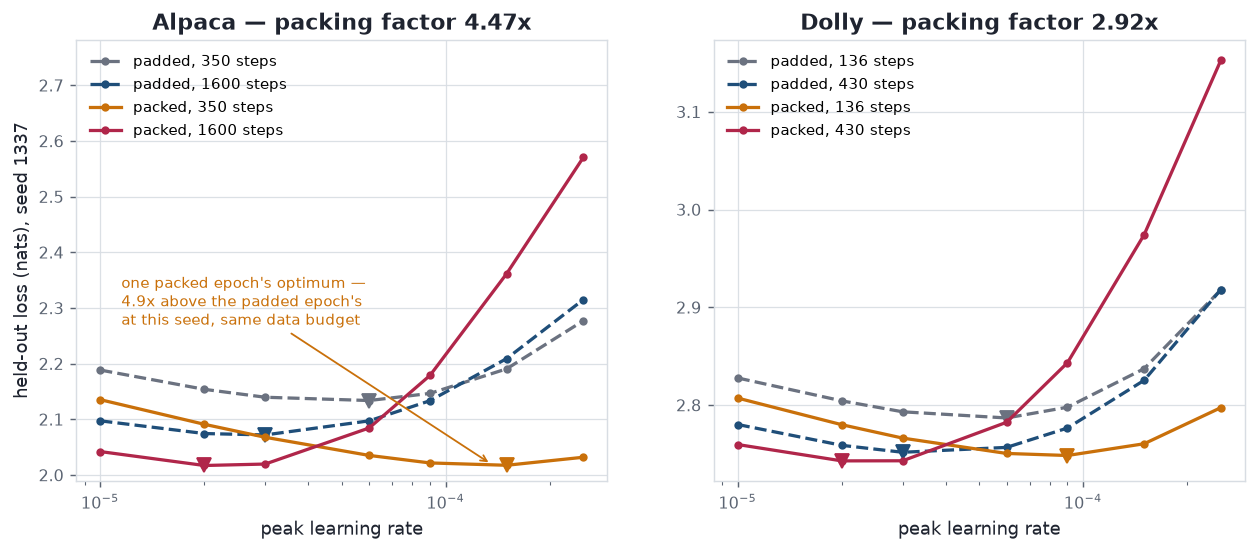
\includegraphics[width=\linewidth]{figures/06-lr-scaling-packing.png}
\caption{Held-out loss against peak learning rate, seed 1337, minima marked. Dashed is padded, solid is packed. The figure is one seed because the held-out split is seeded with the training seed (3.1); the optima in the tables are aggregated across seeds, each solved on its own curve.}
\end{figure}

\subsection{The second corpus, and a prediction that failed}

Section 4.1's exponents were fitted on Alpaca. Dolly is the out-of-sample test: a different corpus, a packing factor of 2.92x in supervised tokens per step (568 to 1,658 per micro-batch, measured; note this is \emph{not} the 3.16x ratio of windows, and the token ratio is what the batch effect is defined against).

Before any Dolly run finished, the Alpaca batch exponent as it then stood (0.673, and 0.670 after seed replication) was recorded as predicting a Dolly batch effect of 2.92\textasciicircum{}0.673 = \textbf{2.06x}.

The measured value is \textbf{1.60x}, an exponent of \textbf{0.440} (three seeds).

The prediction fails, and it fails in an informative direction: 1.60x is close to the square-root rule's 1.71x, while Alpaca's 2.73x sits well above its own square-root prediction of 2.11x.

The failure is larger than the noise. Both cells defining Dolly's batch effect were run at three seeds, with max/min spreads of 1.08x and 1.03x; combined geometrically, that is about 1.09x of seed uncertainty on their ratio. The prediction misses by 1.28x, in log terms about \textbf{2.9 times that spread}. Three seeds give a range and not a standard error, so this is a claim about magnitude rather than a significance test; but the miss is several times the scatter we can actually see, which is what separates a failed prediction from a noisy one.

We therefore do not fit a shared power law. Two corpora, each with a well-bracketed and seed-stable optimum, disagree on the exponent by more than their noise. The obvious reading is that the exponent is corpus-dependent; \S{}4.5 tests that reading against five settings and finds it wrong, so we set it aside here and return to it there. \S{}4.6 supplies the reading that replaces it (the two corpora differ in scale by 3.7x, and matched on scale they agree), but that is a reading arrived at afterwards, and this section reports the prediction as it stood when it failed.

\begin{center}
\small
\setbox0=\hbox{%
\begin{tabular}{lrr}
\toprule
 & Alpaca & Dolly \\
\midrule
packing factor (supervised tokens/step) & 4.47x & 2.92x \\
batch effect at matched steps & 2.73x & 1.60x \\
--- as an exponent & \textbf{0.670} & \textbf{0.440} \\
step effect, padded & 1.78x & 1.29x \\
--- as an exponent & 0.379 & 0.224 \\
matched data budget (one epoch each) & 4.86x & 2.07x \\
--- as an exponent & \textbf{1.055} & \textbf{0.681} \\
worst per-cell seed spread & 1.17x & 1.11x \\
\bottomrule
\end{tabular}}
\ifdim\wd0>\linewidth\resizebox{\linewidth}{!}{\usebox0}\else\usebox0\fi
\end{center}

We do not think the honest reading of this is that one corpus is anomalous. The fixed-step comparison that defines the batch effect necessarily varies data seen as well (at a fixed step count the larger batch consumes proportionally more of the corpus), and that residual confound grows with the packing factor, which is larger for Alpaca. Some part of the exponent gap is therefore built into the design rather than into the models. Li et al.'s (2024) non-monotone picture supplies another candidate: a local exponent that depends on where a batch size sits relative to the gradient noise scale need not be shared by two corpora with different example lengths.

Either way, the conclusion is the same: \textbf{the shift is real and large on both corpora, and it is not described by one exponent.} \S{}4.5 takes up what does describe it.

\subsection{What does replicate}

Three things hold on both corpora.

\textbf{The optimum moves a long way at a matched data budget}: 4.86x on Alpaca and 2.07x on Dolly, against packing factors of 4.47x and 2.92x. Neither is close to the 1.0x that inheriting a learning rate assumes, and both are many times the seed spread.

\textbf{Inheriting the learning rate gives up most of what packing offers.} Taking each corpus's padded optimum (3e-5 on both) and applying it unchanged to the packed run at the same data budget:

\begin{center}
\small
\setbox0=\hbox{%
\begin{tabular}{lrrr}
\toprule
 & padded at its optimum & packed, inherited & packed at its optimum \\
\midrule
Alpaca & 2.0720 (3e-5) & 2.0678 (3e-5) & \textbf{2.0175} (1.5e-4) \\
Dolly & 2.7517 (3e-5) & 2.7662 (3e-5) & \textbf{2.7484} (9e-5) \\
\bottomrule
\end{tabular}}
\ifdim\wd0>\linewidth\resizebox{\linewidth}{!}{\usebox0}\else\usebox0\fi
\end{center}

Retuning is worth \textbf{0.050 nats on Alpaca and 0.018 on Dolly} against inheriting. Measured against the padded baseline instead, the packed run at its own optimum wins on both corpora, by 0.054 and 0.003 nats, while the packed run at the inherited rate wins on neither: 0.004 nats better than padding on Alpaca, which at this scale is a wash, and 0.015 nats \emph{worse} on Dolly. A practitioner who turns packing on and changes nothing else buys throughput and collects, at best, none of the quality packing had available; on one of the two corpora they pay for it.

That gain does not transfer, and it reverses. Registered before any of it existed (\texttt{results/\allowbreak{}registered-prediction-downstream.md}), the three conditions above were re-run with their checkpoints kept (they reproduce the losses in this table to 0.0000 nats) and scored on Dolly's held-out split, which none of them was fine-tuned on, every checkpoint in one invocation so the columns see the same examples. The prediction of record was that the retuned run would still beat the inherited one out of distribution, by more than a fifth of the in-distribution gain. \textbf{It loses by 0.087 nats, where it wins by 0.050 on Alpaca.}

\begin{center}
\small
\setbox0=\hbox{%
\begin{tabular}{lrr}
\toprule
 & Alpaca held-out & Dolly held-out \\
\midrule
base model, no fine-tune & 2.5711 & 3.0653 \\
padded at its optimum & 2.0720 & 2.9518 \\
packed, inherited rate & 2.0678 & \textbf{2.8873} \\
packed, retuned rate & \textbf{2.0175} & 2.9739 \\
\bottomrule
\end{tabular}}
\ifdim\wd0>\linewidth\resizebox{\linewidth}{!}{\usebox0}\else\usebox0\fi
\end{center}

The same comparison reverses sign between the two corpora, and by more than the gain it reverses. On Dolly the ranking puts the \emph{inherited} run first of the three fine-tunes: the condition this section describes as collecting none of the quality packing had available is the one that generalises best of them.

What that costs this section is its practical framing and not its measurement. The 0.050 nats is real and it reproduces exactly; it is a gain \emph{on the corpus being tuned}, which is what \S{}5 says every number in this paper is, and it does not survive a change of distribution. A mechanism is available and is not tested here: the retuned run trains at five times the inherited rate, so it moves further from the base model and specialises harder on what it sees; "specialised harder" and "generalises worse" are the same observation twice. One training seed, as everywhere in this section, and Dolly is a second instruction corpus rather than a downstream task, so this is transfer between instruction distributions and not performance on anything a user would ask for.

The Alpaca column is where this effect is easiest to overstate, so it is worth reading closely. One grid point below the inherited rate, at 2e-5, the packed run scores 2.0911 against padding's 2.0745, a clear regression. The sign of the inherit-versus-padding comparison therefore turns over between two adjacent grid points, which is why we call it a wash on Alpaca rather than a regression, and why the claim we would defend is the 0.050 nats that retuning recovers and not the sign of a difference an order of magnitude smaller. For a change routinely described as pure throughput, that is still the result: packing's quality effect has the sign of its learning rate, not of packing.

One caution about how to read those three numbers together. The batch effect, the step effect and the matched-budget shift are three views of the same four optima, not three independent measurements. At a fixed data budget the step count is the corpus size over the batch size, so the budget shift is fixed once the other two are known: in logs it is their weighted sum, with the weight being the step ratio over the token ratio. Their agreeing with each other is arithmetic and not corroboration, and only the seed replication in Appendix C speaks to whether any of them is more than noise.

\textbf{Step count matters independently of batch size.} Holding the padded batch fixed and changing only the number of optimizer steps moves the optimum 1.78x (Alpaca) and 1.29x (Dolly). Whatever the right functional form, the shift a practitioner sees when turning packing on is not attributable to batch size alone, because packing changes both.

\subsection{Is it the batch, or is it the packing?}

Everything so far treats packing as a way of changing the batch size, and \S{}3.1 argues on the basis of the loss normalization that this is what it is. The factorial cannot check that argument, because in all four of its cells the batch is changed by packing and by nothing else. Packing moves two things at once that a batch-size rule might key on: it multiplies supervised tokens and examples per step by \texttt{p}, and it leaves the number of forward-pass rows per step unchanged. Those come apart if the same batch is assembled the other way.

So we assemble it the other way. Leaving packing off and raising gradient accumulation gives a padded step that matches the packed step on everything a batch-size rule could depend on:

\begin{center}
\small
\setbox0=\hbox{%
\begin{tabular}{lrrrr}
\toprule
cell & supervised tokens/step & examples/step & rows/step & data seen \\
\midrule
Alpaca \texttt{packed\_\allowbreak{}350} & 8,444 & 143 & 32 & 0.98 epoch \\
Alpaca \texttt{wide\_\allowbreak{}350} (accum 18) & 8,496 & 144 & \textbf{144} & 0.99 epoch \\
Dolly \texttt{packed\_\allowbreak{}136} & 6,632 & 93 & 32 & 0.92 epoch \\
Dolly \texttt{wide\_\allowbreak{}136} (accum 12) & 6,816 & 96 & \textbf{96} & 0.95 epoch \\
\bottomrule
\end{tabular}}
\ifdim\wd0>\linewidth\resizebox{\linewidth}{!}{\usebox0}\else\usebox0\fi
\end{center}

The match is within 0.6\% on Alpaca and 2.8\% on Dolly, where the accumulation count is a coarser lever. The two arms differ only in whether those examples arrive packed into shared windows or padded into their own, which costs the padded arm several times the forward-pass rows for the same gradient and is the entire reason packing exists.

\begin{figure}[htbp]
\centering
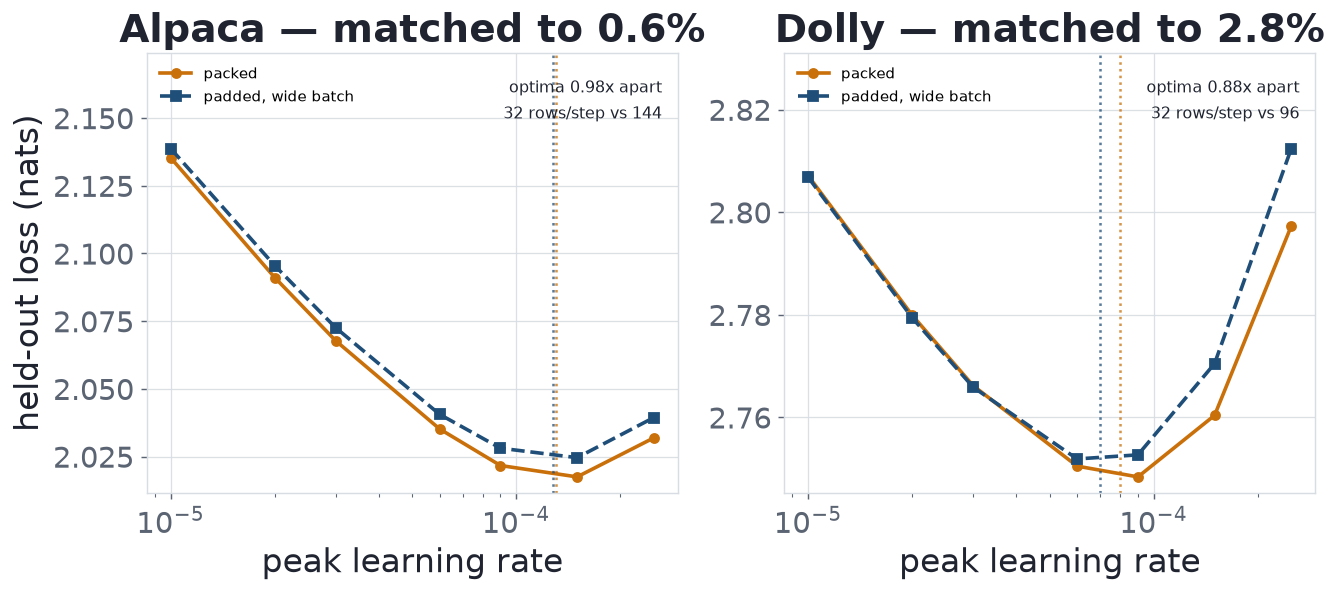
\includegraphics[width=\linewidth]{figures/07-lr-scaling-control.png}
\caption{The same batch, assembled by packing (solid) and by gradient accumulation (dashed), on both corpora. Dotted verticals mark each cell's interpolated optimum. Seed 1337, the seed the two cells share.}
\end{figure}

\begin{center}
\small
\setbox0=\hbox{%
\begin{tabular}{lrrrrr}
\toprule
 & packed lr* & wide lr* & ratio & batch rule predicts & rows rule predicts \\
\midrule
Alpaca & 1.30e-4 & 1.28e-4 & \textbf{0.98x} & 1.00x & 4.47x \\
Dolly & 7.98e-5 & 7.00e-5 & \textbf{0.88x} & 1.00x & 2.92x \\
\bottomrule
\end{tabular}}
\ifdim\wd0>\linewidth\resizebox{\linewidth}{!}{\usebox0}\else\usebox0\fi
\end{center}

The rows rule is dead on both corpora, rejected by factors of 4.6 and 3.3. Running several times the forward-pass rows for the same gradient does not move the optimum anywhere near that far, so the optimum is set by the examples the step carries, not by how many sequences the forward pass processes. \textbf{Packing's effect on the learning rate is a batch-size effect, and the identical optimum is reachable without packing at all, by padding, at several times the compute.} That is what makes the rest of this paper a result about batch size which packing is a convenient way of changing, rather than a result about a representation.

The batch rule is matched closely but not exactly, and the two corpora differ in how closely. Alpaca's 0.98x sits inside that cell's seed spread of 1.11x, so the match is as exact as this evidence can resolve. Dolly's 0.88x sits outside its much tighter spread of 1.03x, and Dolly's 2.8\% batch mismatch runs the wrong way to explain it: a slightly \emph{larger} wide batch should put its optimum slightly above the packed one, not 12\% below.

The residual has a visible shape. The padded arm's loss relative to the packed arm rises with the learning rate on both corpora. On Alpaca it is positive throughout and strictly monotone, from +0.0034 nats at 1e-5 to +0.0075 at 2.5e-4. On Dolly it starts marginally negative (the padded arm is better by 0.0003 to 0.0005 nats over the bottom three points), crosses over between 3e-5 and 6e-5, and then climbs steeply to +0.0151. A penalty that grows with the rate pushes the padded arm's optimum down, which is the direction of both deviations and why Dolly's, with much the steeper climb, is the larger.

We do not have an explanation for that penalty, and two candidates do not survive checking. It is not the loss normalization: averaging the token-mean over 18 accumulation groups rather than 4 would weight tokens unevenly only if the groups were unevenly sized, and the two arms' supervised tokens per micro-batch vary by almost the same relative amount (coefficient of variation 0.35 padded against 0.38 packed). It is not an ordering effect from bin packing either: best-fit-decreasing groups similar-length examples into a window, but the loader shuffles windows, so no length curriculum survives to training. What can be said is that the effect is small, that its direction biases the measured ratio below 1.00x, and that it therefore makes the agreement look worse than it is rather than better.

One further caveat: each wide cell is a single seed. The control was run to answer a question whose two hypotheses differ by a factor of three to four and a half, which one seed settles; it was not run to resolve a 12\% residual, and does not.

\subsection{What the exponent is not a function of}

\S{}4.2 leaves the exponent disagreeing between two corpora, and the obvious reading is that it is corpus-dependent. Two corpora cannot support that: Alpaca and Dolly differ in packing ratio and in everything else about them at once, so "depends on the corpus" and "depends on the packing ratio" fit the same two numbers equally well. Separating them needs a packing ratio that moves while the corpus does not.

Splitting one corpus by length gives that. Sorted by encoded length, Alpaca's terciles are an exact partition (3 x 17,302 = 51,906 usable examples) and pack at 7.85x, 4.87x and 2.73x against the whole corpus's 4.53x. Each tercile holds the same 16,956 training examples and runs the same 530 padded steps, and every cell is one epoch by construction, so each row is the same confound-free matched-budget comparison as \S{}4.3's.

\begin{center}
\small
\setbox0=\hbox{%
\begin{tabular}{lrrrrr}
\toprule
corpus & packing factor & lr* padded & lr* packed & shift & exponent \\
\midrule
Alpaca short third & 7.84x & 4.80e-5 & 1.39e-4 & 2.90x & \textbf{0.517 $\pm$ 0.042} \\
Alpaca middle third & 4.87x & 4.48e-5 & 1.33e-4 & 2.96x & \textbf{0.651 $\pm$ 0.133} \\
Alpaca long third & 2.73x & 6.73e-5 & 1.37e-4 & 2.03x & \textbf{0.707 $\pm$ 0.265} \\
Alpaca, whole & 4.47x & 2.81e-5 & 1.37e-4 & 4.86x & \textbf{1.055 $\pm$ 0.128} \\
Dolly & 2.92x & 3.78e-5 & 7.84e-5 & 2.07x & \textbf{0.681 $\pm$ 0.099} \\
\bottomrule
\end{tabular}}
\ifdim\wd0>\linewidth\resizebox{\linewidth}{!}{\usebox0}\else\usebox0\fi
\end{center}

Each bound carries both cells' seed spreads through the ratio. It is built from max/min ranges rather than standard errors, so with three seeds it is roughly 1.7 standard deviations and deliberately conservative. Reporting it changes what this table supports, and we state the comparisons against it rather than against the point estimates.

The corpus is not it. Two \emph{different} corpora at similar packing ratios, the long tercile at 2.73x and Dolly at 2.92x, differ by 0.026 against a combined bound of 0.282. They are indistinguishable. That is the wrong way round for corpus identity setting the exponent, though it is weak evidence: the pair is matched on nothing else either, and the long tercile's bound is wide enough to hide a real difference.

The packing ratio is not established as it either. Across the three terciles the exponent spans 0.191, from 0.517 to 0.707. The combined bound on those two ends is 0.268, so the spread is 0.7x its own noise. This is the one comparison in the paper whose verdict moves appreciably with how the shift is summarised, because it is the one that spans the widest range of packing factors, 2.87x (\S{}3.3). Under a linear normalization the same spread is 1.01x its noise rather than 0.71x, and under a square-root-relative one it is 0.57x and not monotone. Unsupported under all three, then, but only just under one, and we report the weakest of them rather than the most convenient (Appendix G). The point estimates fall in a tidy monotone order (the exponent decreasing as the packing ratio rises), and that order does not survive the seed spread. We report the trend as unsupported rather than as a finding, and note that it \emph{was} a finding until the terciles were replicated.

Splitting by length also cannot move the packing ratio alone, because the ratio \emph{is} a function of the lengths: across the three terciles the padded step carries 411, 1,334 and 3,709 supervised tokens, a ninefold range, and the mean response length runs 13 to 116 tokens. The task changes with the ratio, which is why the next section changes scale instead, holding composition fixed.

\subsection{What it is a function of}

The one comparison in \S{}4.5's table that clears its bound is between a corpus and a third of itself. That was reached by elimination, so we tested it. Before any run existed we registered a prediction (\texttt{results/\allowbreak{}registered-prediction-scale.md}): a \emph{random} third of Alpaca, matched to the whole corpus on packing factor (4.51x against 4.47x), on supervised tokens per padded step (1,841 against 1,888) and on length distribution, and differing only in scale, should land near 0.67 if scale governs and near 1.055 if it does not.

It measures \textbf{0.670 $\pm$ 0.043} over three seeds, against a registered 0.67.

One comparison falls out of that unplanned. The middle \emph{length tercile} sits at 0.651 and the \emph{random} third at 0.670, inside either one's bound. They share size (16,956 examples) and step count (530) and differ in packing ratio (4.87x against 4.51x) and in composition. Two subsets matched on scale and differing in ratio and composition agree; a subset and its parent matched on ratio and composition and differing in scale do not.

Extending to a third point, with everything but scale held:

\begin{center}
\small
\setbox0=\hbox{%
\begin{tabular}{lrrrrrr}
\toprule
corpus & examples & padded steps & packing & exponent & batch term & step term \\
\midrule
Alpaca ninth & 5,652 & 177 & 4.53x & \textbf{0.412 $\pm$ 0.136} & 0.350 & 0.062 \\
Alpaca third & 16,956 & 530 & 4.51x & \textbf{0.670 $\pm$ 0.043} & 0.520 & 0.150 \\
Alpaca, whole & 50,868 & 1,600 & 4.47x & \textbf{1.055 $\pm$ 0.128} & 0.670 & 0.385 \\
\bottomrule
\end{tabular}}
\ifdim\wd0>\linewidth\resizebox{\linewidth}{!}{\usebox0}\else\usebox0\fi
\end{center}

The exponent rises monotonically across a ninefold span of scale, and both steps clear their combined bounds, 1.8x and 2.9x. So does each of the two terms it decomposes into. That decomposition is worth stating on its own: at a fixed data budget the exponent is a batch term plus a step term (\S{}4.3), and running the padded arm at the \emph{packed} step count isolates the first. Both fall at smaller scale, and the step term falls faster: from the whole corpus down to a ninth the batch term drops to 0.52 of its value and the step term to 0.16. \textbf{The scale effect is not localised in the batch term}, which is what a rule about batch size alone would have predicted. A shorter run is less sensitive to both levers, and at the smallest scale here the step count has nearly stopped mattering.

\begin{figure}[htbp]
\centering
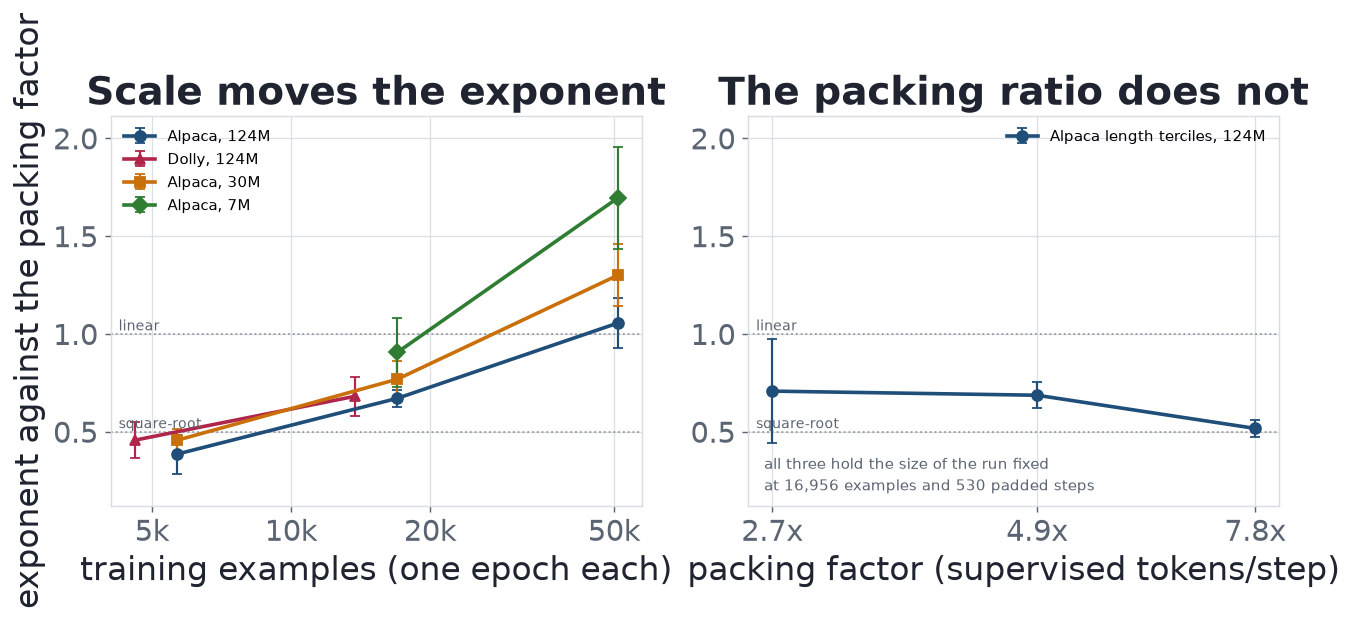
\includegraphics[width=\linewidth]{figures/08-lr-scaling-regime.png}
\caption{Left: the exponent against the size of the run, with packing factor, padded batch and length distribution held, on both corpora and, from \S{}4.7, at all three model sizes. Every series rises, and the smaller the model the higher it sits, though adjacent models' bars overlap and only the 124M-to-7M span separates. Right: the exponent against the packing factor across Alpaca's three length terciles, which hold the size of the run fixed instead. Error bars are the seed bound of \S{}4.5, both cells' ranges carried through the ratio and so conservative. The right-hand panel is why they are drawn: without them its three points look like a trend.}
\end{figure}

It replicates on the second corpus. A second prediction was registered before the runs existed, this time directional: a random third of Dolly should land below the whole corpus by more than the combined bound. Dolly's whole corpus is 0.681 $\pm$ 0.099 and its third is \textbf{0.456 $\pm$ 0.092}, a gap of 0.225 against a bound of 0.135, or 1.7x. Alpaca's threefold scale step moves the exponent 0.385 and Dolly's moves it 0.225, on corpora differing in size, packing ratio and provenance.

It also explains the prediction that failed in \S{}4.2, and it does so across corpora rather than within one. That prediction assumed Alpaca and Dolly share an exponent. They do not, and on this section's reading they should not: the two corpora differ in scale by 3.7x, 50,868 training examples against 13,756. Match the scale and the disagreement goes away.

\begin{center}
\small
\setbox0=\hbox{%
\begin{tabular}{lrrr}
\toprule
corpus & examples & packing factor & exponent \\
\midrule
Alpaca, random third & 16,956 & 4.51x & 0.670 $\pm$ 0.043 \\
Dolly, whole & 13,756 & 2.92x & 0.681 $\pm$ 0.099 \\
Alpaca, random ninth & 5,652 & 4.53x & 0.412 $\pm$ 0.136 \\
Dolly, random third & 4,585 & 3.14x & 0.456 $\pm$ 0.092 \\
\bottomrule
\end{tabular}}
\ifdim\wd0>\linewidth\resizebox{\linewidth}{!}{\usebox0}\else\usebox0\fi
\end{center}

Two corpora of different provenance and length distribution, differing by about half again in packing ratio and matched only to within 1.23x on the size of the run, agree on the exponent at \textbf{both} scales: by 0.011 against a bound of 0.108, and by 0.044 against 0.164, or 0.10x and 0.27x of their own noise. One corpus moved 3x in scale disagrees with \emph{itself} by 2.85x its bound. Matching the scale makes two different corpora agree; changing it makes one corpus disagree with itself.

These two are worth more than the rest of this section's comparisons for a reason \S{}5 gives: every other scale comparison here is a corpus against a nested subset of itself, so a property of that corpus cannot show up as variation. These are between corpora. The only other cross-corpus pair in the paper is \S{}4.5's long tercile against Dolly, and that one is matched on packing ratio rather than on scale, so between them the two sections check the same independence on both axes, and it holds on both.

They are weaker individually than that framing suggests. The scales are matched to within 1.23x rather than exactly, Dolly's bounds are the widest of any whole-corpus cell, and two pairs are two pairs: agreement inside a bound this size is a test the scale reading could have failed and did not, rather than a demonstration that the exponent is a function of scale alone.

These two pairs are also the ones most exposed to how the shift is summarised, because unlike every other comparison in \S{}4.6 and \S{}4.7 they do not hold the packing factor fixed: 4.51x against 2.92x, and 4.53x against 3.14x (\S{}3.3). The agreement survives under two alternative normalizations, at 0.50x and 0.51x of the bound rather than 0.10x, so the conclusion does not depend on the choice; the \emph{closeness} partly does. Appendix G gives the table.

\textbf{A retraction worth reporting.} Before replication the three Alpaca points sat exactly 3x apart in scale with exponent differences of +0.369 and +0.371, a straight line in log(scale) with residuals of $\pm$0.0006. We declined to call it a law at the time, on the grounds that residuals two orders of magnitude below the seed bounds are coincidence rather than signal. Replication settles it: the differences are now \textbf{+0.258 and +0.385} and the line is gone. The monotone increase survives, at roughly 0.3 of exponent per tripling of scale, with no functional form behind it. We report this because the tidy version was available for several hours and would have been the more quotable result.

Two limits remain. The three Alpaca samples are nested, so these are a set and its supersets rather than independent draws. And "scale" is not one variable: a larger corpus at one epoch means both more data and more optimizer steps, and at a fixed data budget those are the same quantity, so nothing here separates them. Li et al. (2024) place the dependence on where the batch sits relative to the gradient noise scale. We could not measure where ours sit well enough to quote a number (the three settings that share a distribution disagree by 1.55x), but every fit puts the packed arm several times above the scale rather than below it (\texttt{results/\allowbreak{}noise-scale.md}), which is the opposite of what \S{}2 assumes.

\subsection{Three model sizes}

Every result so far is one model. To test whether any of it survives a change of scale in the model rather than in the data, we pretrained two more on the same FineWeb-Edu corpus with the same architecture: 30M parameters (\texttt{small}, d\_model 384, 6 layers) and 7M (\texttt{mini}, d\_model 128, 4 layers). With the 123.6M model that is three sizes about 4x apart, spanning 17x. Every hyperparameter that could confound a size comparison is held at the 124M run's value, and the fine-tuning window is fixed at 512 tokens in all three, so the packing factors, the per-step supervised-token counts and the cell step counts carry over unchanged: the only thing that differs between the factorials is the base model.

The intent was to match the three on tokens per parameter rather than on absolute tokens, so that each would be comparably trained \emph{for its size}. The budget we set does not do that, and the error is worth stating plainly because it changes what the comparison below means. The 124M run saw 2.46B tokens (19.9 per parameter) and both smaller runs were sized from a stale note that assumed twice that: 1.18B tokens at 30M and 288M at 7M, or 39.4 and 39.5 per parameter. Both smaller models are therefore trained about twice as heavily for their size as the model they are being compared against, which would confound \emph{better-trained-for-its-size} with \emph{smaller} throughout this section. \S{}4.7.1 measures that axis directly at 30M rather than leaving it as a caveat, and finds it null; the rest of this section is written on that basis. Validation perplexities are 23.5, 38.0 and 115.2.

Repeating the scale series of \S{}4.6 at each size. Three seeds stand behind every cell here, including the 124M ninth, whose window Appendix C records as having been extended to get there; none of the fourteen cells added at 30M and 7M lost a seed:

\begin{center}
\small
\setbox0=\hbox{%
\begin{tabular}{lrrrr}
\toprule
corpus & examples & 124M & 30M & 7M \\
\midrule
Alpaca ninth & 5,652 & 0.412 $\pm$ 0.136 & 0.456 $\pm$ 0.059 & --- \\
Alpaca third & 16,956 & 0.670 $\pm$ 0.043 & 0.768 $\pm$ 0.094 & 0.905 $\pm$ 0.174 \\
Alpaca whole & 50,868 & 1.055 $\pm$ 0.128 & 1.300 $\pm$ 0.159 & \textbf{1.695 $\pm$ 0.261} \\
\bottomrule
\end{tabular}}
\ifdim\wd0>\linewidth\resizebox{\linewidth}{!}{\usebox0}\else\usebox0\fi
\end{center}

The effect is not a 124M artefact, and it grows as the model shrinks. One packed epoch of Alpaca wants 4.86x the padded learning rate at 124M, 7.01x at 30M and \textbf{12.66x} at 7M, the largest shift measured anywhere in this paper, from 1.19e-4 padded to 1.51e-3 packed. The cost of ignoring it grows with it. Taking each model's padded optimum and inheriting it into the packed run at the same data budget, retuning is worth 0.050 nats at 124M, 0.110 at 30M and \textbf{0.172} at 7M. Whatever a practitioner loses by inheriting a learning rate through a packing change, they lose more of it on a smaller model.

The left panel of the figure in \S{}4.6 draws all three sizes together.

The scale dependence replicates at every model size, and the first replication was registered before it ran. Within each model the whole corpus sits above a third of it by more than the combined seed bound: 2.8x at 124M, 2.9x at 30M, 2.5x at 7M. Against a ninth, where we have two of the three sizes, it is 3.4x and 5.0x. Five comparisons on three base models, and \S{}4.7.1 adds a fourth base model and a sixth. This is the paper's most repeated result and the one we would defend hardest.

The 30M case is the fourth registered prediction in this paper and the third confirmed (\texttt{results/\allowbreak{}registered-prediction-model-size.md}, written while the 30M pretraining run was still going and before any 30M fine-tune existed). It committed to direction plus margin rather than to values: that Alpaca's exponent would exceed its third's \emph{by more than 0.135}, the combined bound at 124M, with the alternative on record that a gap under 0.135 in either direction would mean \S{}4.6's scale reading had to be reported as 124M-specific. The measured gap is 0.531. That document also recorded, as an explicit limitation, that the 30M sweep as queued ran seed 1337 only and so would carry no seed bound of its own until replicated; the replication was run afterwards and is in Appendix C, and it did not move the verdict.

Model size moves the exponent across the full span, but not between adjacent sizes. Every point estimate is ordered the same way (all six pairs, on both corpus sizes, put the smaller model higher), and one comparison clears its bound: 1.695 against 1.055 on the whole corpus, a gap of 0.640 against 0.291, or 2.2x across 17x of model size. Nothing else does. The adjacent steps are 1.2x and 1.3x of their bounds on the whole corpus, and on the third the whole 17x span reaches only 1.3x. So the direction is consistent across six comparisons and the magnitude is resolved in one of them; three sizes at three seeds cannot do better than that, and we state the claim at the span rather than at the step.

"Model size" here means size and quality together, and this design cannot separate them. A smaller model trained on the same corpus is a worse model: validation perplexities are 23.5, 38.0 and 115.2 across the three. So every comparison in this section moves parameter count and base-model quality at once, and the claim above could as easily be read as \emph{the exponent rises as the base model gets worse}. \S{}4.7.1 is the only evidence that bears on it, and it is suggestive rather than sufficient: the exponent is flat across a 38.0-to-43.9 change in perplexity at fixed size, but the gap this question concerns is a factor of five, not fifteen per cent.

The confound is separable, because the 124M pretraining run checkpointed every 500 steps and its perplexity trajectory passes through the other two models' final values. \S{}4.7.2 runs that control on the extreme point of it (a 124M model at the 7M model's perplexity) against a prediction registered before the runs existed. The exponent stays with the parameter count, so the reading in this section is a reading about model size, and the abstract and contribution 7 say so too.

One thing that does not replicate is the sign of the inherit-versus-padding comparison. At 7M the inherited rate beats padding by 0.038 nats, where at 124M on Dolly and at 30M it loses by 0.015 and 0.009. \S{}4.3 already reports that sign turning over between two adjacent grid points on Alpaca, and three model sizes now put it on both sides. The distance from the inherited rate to the retuned one (0.050, 0.110, 0.172 nats) is the quantity that is stable in direction and grows with every step down in model size.

\subsubsection{The pretraining budget is not what moves it}

The budget error above leaves every size comparison confounded, so we measured the confound rather than arguing about it. The 30M run checkpointed every 500 steps, and step 9,000 (590M tokens, 19.7 per parameter against the 124M run's 19.9) is the same model at the budget the comparison was meant to use. It is a visibly worse base model than the one at step 18,000: validation perplexity 43.9 against 38.0. The 7M run gives the same control at a second size: its step 2,000 is 18.0 tokens per parameter against the final checkpoint's 39.5, at perplexity 142.4 against 115.2. Repeating both comparisons from both, three seeds each:

\begin{center}
\small
\setbox0=\hbox{%
\begin{tabular}{llrrrr}
\toprule
base model & corpus & lr* padded & lr* packed & shift & exponent \\
\midrule
30M, 39.4 tokens/param & Alpaca third & 6.31e-5 & 2.01e-4 & 3.18x & 0.768 $\pm$ 0.094 \\
30M, 19.7 tokens/param & Alpaca third & 9.19e-5 & 3.01e-4 & 3.27x & 0.787 $\pm$ 0.100 \\
30M, 39.4 tokens/param & Alpaca whole & 3.50e-5 & 2.45e-4 & 7.01x & 1.300 $\pm$ 0.159 \\
30M, 19.7 tokens/param & Alpaca whole & 5.06e-5 & 3.56e-4 & 7.03x & 1.302 $\pm$ 0.119 \\
7M, 39.5 tokens/param & Alpaca third & 1.89e-4 & 7.39e-4 & 3.91x & 0.905 $\pm$ 0.174 \\
7M, 18.0 tokens/param & Alpaca third & 2.73e-4 & 1.04e-3 & 3.80x & 0.886 $\pm$ 0.201 \\
7M, 39.5 tokens/param & Alpaca whole & 1.19e-4 & 1.51e-3 & 12.66x & 1.695 $\pm$ 0.261 \\
7M, 18.0 tokens/param & Alpaca whole & 2.19e-4 & 2.38e-3 & 10.85x & 1.592 $\pm$ 0.333 \\
\bottomrule
\end{tabular}}
\ifdim\wd0>\linewidth\resizebox{\linewidth}{!}{\usebox0}\else\usebox0\fi
\end{center}

Halving the pretraining budget does not move the exponent. The four pairs differ by 0.019, 0.002, 0.019 and 0.103 against combined bounds of 0.137, 0.198, 0.266 and 0.424, between 0.0x and 0.2x of their own noise, and the smallest differences anywhere in this paper. Doubling how heavily the base model is trained for its size leaves how far packing moves the optimum where it was, and it does so at both model sizes this could be checked at.

It does move both optima, and by the same factor. All eight learning rates rise when the base model is the less-trained one, and within each pair they rise together: 1.46x and 1.50x on the 30M third, 1.45x and 1.45x on the 30M whole corpus, 1.44x and 1.40x on the 7M third, 1.84x and 1.57x on the 7M whole corpus. A less-pretrained model wants a larger fine-tuning step in both arms, and the \emph{distance} between the arms (the only quantity this paper measures) is untouched. The exponent is therefore not inherited from how well the base model was trained, which is what makes \S{}4.7's size comparison a comparison of sizes rather than of budgets in disguise. It also means a practitioner cannot read their own optimum off ours: where the optimum sits depends on the base model, while how far it moves does not.

The scale dependence survives at both checkpoints too (0.787 against 1.302 is a gap of 0.515 against a bound of 0.155, or 3.3x, and 0.886 against 1.592 is 0.706 against 0.389, or 1.8x), which makes it five base models in a row (\S{}4.6, \S{}4.7) on which a third of the corpus wants a smaller exponent than the whole of it.

What this does not settle is the shape of the budget axis. It is two model sizes, each at two budgets about a factor of two apart, all four far below where a model of that size would be trained in practice; it establishes that the exponent is flat across those intervals and not that it is flat everywhere. The 7M whole-corpus pair is also the widest-bounded comparison in the paper (its padded cell spreads 1.62x across seeds, the largest anywhere), so it is the weakest of the four even though it agrees with them.

\subsubsection{Model size, or model quality?}

The comparison above moves two things at once. A smaller model trained on the same corpus is also a worse model (validation perplexities are 23.5, 38.0 and 115.2 across the three sizes), so \emph{smaller} and \emph{worse} are perfectly confounded in it, and the trend has a second reading in which the exponent tracks not parameter count but how badly the base model models language.

The confound is separable because the 124M pretraining run checkpointed every 500 steps, and its perplexity trajectory passes through the smaller models' final values. Fine-tuning the whole-Alpaca factorial from \texttt{step\_\allowbreak{}500}, at perplexity 107.0 against the 7M model's 115.2, gives a 124M model \emph{at the 7M model's quality}. Everything else is held: the same architecture, the same window, the same 4.47x packing factor, the same two cells, the same estimator and the same three seeds. The prediction was registered before any run of it existed (\texttt{results/\allowbreak{}registered-prediction-size-vs-quality.md}), with H1 (that the exponent tracks parameter count) as the prediction of record: it should land near the 124M value of 1.055 and more than 0.291 below 7M's 1.695, that margin being the combined seed bound \S{}4.7 already reports for the pair.

\begin{center}
\small
\setbox0=\hbox{%
\begin{tabular}{lrrrrr}
\toprule
base model & perplexity & lr* padded & lr* packed & shift & exponent \\
\midrule
124M, step 20,000 & 23.5 & 2.81e-5 & 1.37e-4 & 4.86x & 1.055 $\pm$ 0.128 \\
124M, step 2,500 & 39.4 & 5.22e-5 & 2.85e-4 & 5.46x & 1.133 $\pm$ 0.107 \\
124M, step 500 & 107.0 & 1.12e-4 & 4.36e-4 & 3.89x & 0.906 $\pm$ 0.204 \\
7M, final & 115.2 & 1.19e-4 & 1.51e-3 & 12.66x & 1.695 $\pm$ 0.261 \\
\bottomrule
\end{tabular}}
\ifdim\wd0>\linewidth\resizebox{\linewidth}{!}{\usebox0}\else\usebox0\fi
\end{center}

The exponent tracks parameter count, not base-model quality. At the 7M model's perplexity and the 124M model's parameter count it reads 0.906: 0.789 below 7M's 1.695, or 2.7x the registered margin, and 0.149 from the fully pretrained 124M model's own 1.055, against a combined bound of 0.241. Base-model quality was moved by a factor of 4.6 in perplexity and the exponent did not follow it; it stayed with the parameter count. H1 is confirmed on the criterion named in advance, and \S{}4.7's claim is a claim about model size.

The middle of that range was then registered and run, and it holds there too. \texttt{step\_\allowbreak{}2500}, at perplexity 39.4 against the 30M model's 38.0, was predicted in advance to land below 1.178 (the midpoint of 124M's 1.055 and 30M's 1.300) and to leave the three-point series spanning no more than 0.332. It reads \textbf{1.133 $\pm$ 0.107} and the series spans 0.227, so both conditions hold, but the second number is the honest one to quote: it passes the side condition by 0.045, where the \texttt{step\_\allowbreak{}500} point cleared its margin by 2.7x. Two things are worth stating rather than smoothing. The registered point estimate was 1.00 and the measured value sits outside the 0.90--1.10 band that registration named. And the three point estimates run 1.055, 1.133, 0.906 as the base model gets worse, which is \textbf{not monotone}. What holds the reading up is that no pair of the three separates (the gaps are 0.46x, 0.62x and 0.98x of their own combined bounds), so the claim this section makes is that the exponent is flat across a 4.6-fold range of base-model perplexity to within the resolution of this study, and not that it rises and then falls. The widest of those gaps sits at 0.98x of its bound, which is as close to separating as a pair can come without doing so.

It does move both optima, by three to four times. The padded optimum rises 4.00x against the fully pretrained model and the packed one 3.20x, and the midpoint sits between at 1.86x and 2.09x. That is \S{}4.7.1's finding over a much longer range: a less well trained base model wants a larger fine-tuning rate in both arms, while the \emph{distance} between the arms is left where it was. The registration expected this and recorded in advance that it discriminates nothing between the two hypotheses, which it does not. It is reported because it is the practical half: a practitioner reading an optimum off this paper would be wrong by 4x if their base model were as undertrained as this one, while reading the \emph{shift} off it would not.

\begin{figure}[htbp]
\centering
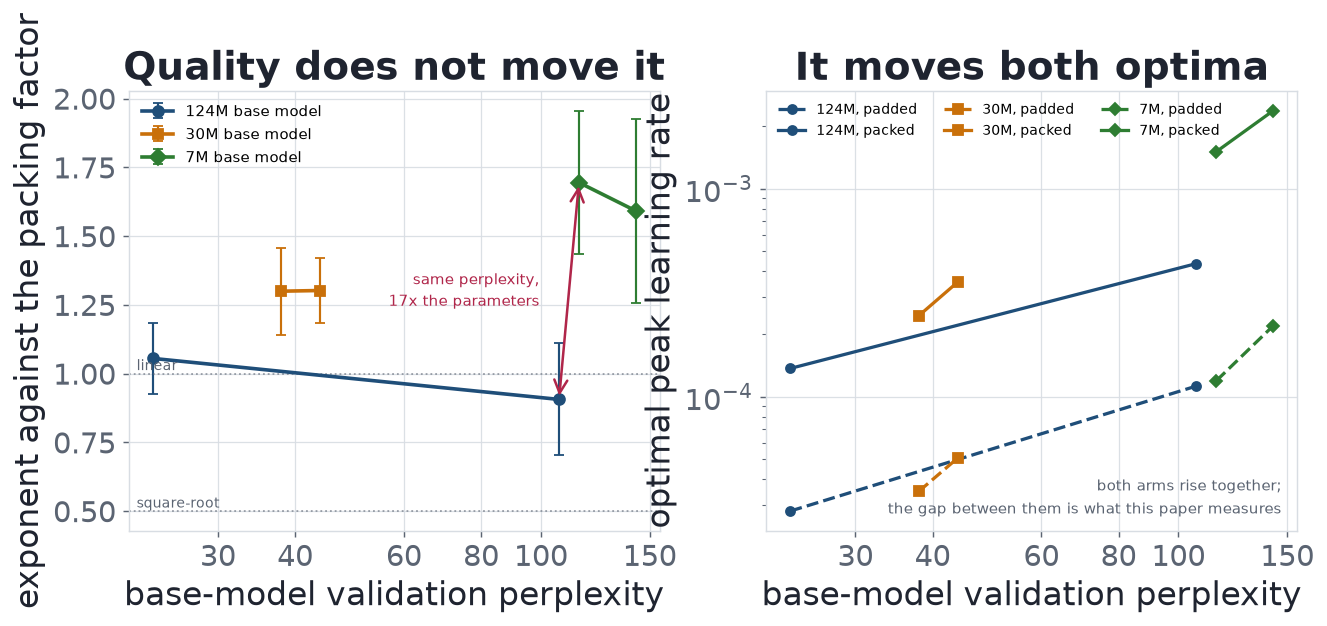
\includegraphics[width=\linewidth]{figures/09-lr-scaling-quality.png}
\caption{Left: the exponent against the base model's validation perplexity. The 124M series spans the whole quality range these three models cover and stays flat, while the 7M model sits at the same perplexity as its worst point and more than half an exponent above it. Right: the optima themselves, on the same axis. Both arms rise together as the base model gets worse, by three to four times over this range, while the distance between them is left where it was. Error bars are the seed bound of \S{}4.5; perplexities are read from each model's own pretraining log.}
\end{figure}

\textbf{What this does not settle}, all of it recorded in the registration before the runs existed. An early checkpoint of a large model is not a converged small one: at step 500 of 20,000 the weights are 2.5\% of the way through a cosine schedule, so matching on perplexity matches one number and not the state, and this is the main reason to read the result as evidence about the confound rather than as its dissolution. Perplexity is also one axis of quality among several, and the two models are matched on held-out FineWeb-Edu loss rather than on any downstream capability. And it is one corpus at one packing factor. The axis now has three points rather than two, but three points an order of magnitude apart in perplexity, none of which separates from the others, constrain the \emph{shape} of the dependence hardly at all: they establish that it is flat at this resolution, not that it is flat.

\section{Threats to validity}

\textbf{Model size was confounded with base-model quality, and the control has two points rather than three.} The three models differ in parameter count and in how well they model language (perplexity 23.5, 38.0 and 115.2), so \S{}4.7's trend had a second reading in which the exponent tracked base-model quality instead. \S{}4.7.1 ruled that out across a small change in quality at fixed size, and \S{}4.7.2 across a factor of 4.6, at the extreme point where a 124M model is taken to the 7M model's perplexity: the exponent stays with the parameter count. The direction is settled and the shape is not. The middle point of the quality series has since been registered and run and it agrees, so the axis has three points; but none of the three separates from the others, so they bound the dependence rather than describing it. And an early checkpoint of a large model is not a converged small model, since matching on perplexity matches one number and not the state of the weights. We read \S{}4.7.2 as evidence about the confound rather than as its dissolution.

\textbf{Three model sizes, two source corpora, and a ratio axis built by subsetting them.} Most numbers come from a 124M model; \S{}4.7 repeats the scale series at 30M and 7M, which makes the model-size axis three points about 4x apart. That is a direction rather than a curve: the ordering is consistent across all six pairwise comparisons, but only the 17x extreme on the whole corpus separates from its seed bound, and three points cannot distinguish the shape of the dependence from a straight line through them. All three sizes are far below any model that would be fine-tuned in practice.

The packing-ratio axis is better covered than it was (eight settings from 2.73x to 7.84x in supervised tokens per step, rather than the two whole corpora at 4.47x and 2.92x that \S{}4.2 rests on), but six of those eight are subsets of the same two corpora, nested within them rather than drawn independently. The three length terciles partition Alpaca; the random ninth and third are a set and its superset; Dolly's third is drawn from Dolly. So the axis is covered by re-slicing two datasets, not by eight datasets, and a property shared by both sources would not show up as variation anywhere in it. The model-size axis re-uses those same subsets, which means \S{}4.7 adds points in model size and none in data: the two axes are not independent, and a corpus artefact would appear at all three sizes rather than cancelling between them.

What that does and does not buy: it is enough to rule the corpus out as what fixes the exponent and to leave the packing ratio unsupported (\S{}4.5), and enough to establish the scale dependence on both corpora (\S{}4.6), because those are comparisons \emph{within} the nesting. Two comparisons escape it (Alpaca's third against Dolly whole, and Alpaca's ninth against Dolly's third, both in \S{}4.6), and they are the only evidence here that survives the objection in full, being between corpora rather than within one. Two pairs are not many. It is not enough to estimate a law. \S{}4.2 is the direct evidence for that caution (the exponent fitted on the first corpus does not predict the second), and \S{}6's bracket is the second, having been falsified out of sample five times over by the smallest-scale settings and by the two smaller models once they existed, most recently by a factor of 2.4. Nothing here constrains behaviour at a model larger than 124M, or at a longer window.

\textbf{Small absolute batch.} At 1,888 and 8,444 supervised tokens per step on Alpaca, and 2,272 and 6,632 on Dolly, both arms are far below the batch sizes at which large-scale scaling rules are usually measured, and Li et al. (2024) predict this is the regime where the square-root rule holds. Our own attempt to measure that scale puts it below both arms rather than far above them, though with too much spread between settings that should agree to quote a value; if that sign is right, the packed arm sits past the peak of Li et al.'s non-monotone optimum rather than in its square-root tail, and the regime this paragraph assumes is not the regime this study ran in. Results here should not be extrapolated to production batch sizes without further points.

\textbf{fp16 dynamic range.} All runs use fp16 autocast with a gradient scaler, so at the top of a grid a rise in validation loss could in principle be overflow rather than too large a step. This matters more than it did once the 7M grids are included, because their optima sit an order of magnitude higher and the sweep runs to 2.5e-3. The logs argue against it at every size: across all 677 run logs in the nine ledgers of Appendix D, all of them rather than a sample, there is no NaN and no infinity in either training or validation loss, at any learning rate in any grid, up to 4.0e-3.

The only steps anywhere that jump more than 50\% above their run's running minimum are the seven in one cell (the short tercile's padded arm), and six of them are at the same step, 490 of 530, at every learning rate in that cell from 2e-5 to 2.5e-4. A jump that is independent of the step size and reproducible at a fixed data order is a property of which examples that batch holds, not of the numerics, and it is in training loss rather than in the validation loss anything here is scored on. The seventh is at that cell's highest rate, 4e-4, and trips the same threshold earlier, at step 180, which is what a genuinely too-large step looks like and is the reason the threshold is worth reporting rather than tuning away. \texttt{scripts/\allowbreak{}check\_\allowbreak{}numerical\_\allowbreak{}stability.py} re-runs all of this. High-learning-rate runs otherwise train smoothly and simply end up worse, which is a too-large step rather than a numerical failure. What this does not rule out is the scaler silently skipping occasional overflowing steps, since the skip count is not logged; the effect of that would be a slightly shorter effective schedule at high learning rates.

\textbf{Packed cells run more epochs at matched step counts.} In the packed 1,600-step cell the model sees 4.50 epochs of Alpaca, and this project has previously measured that Alpaca overfits within a single pass. Where the optimum in that cell is set by overfitting rather than by step size, the validation curves in \S{}4 show it directly.

\textbf{Warmup length co-varies with step count.} Warmup is 6.25\% of the schedule in every cell. That keeps the schedule's \emph{shape} identical across the grid, which is what lets cells differ only in length, but it also means the step effect in \S{}4.3 is measured across cells that warm up over 22 steps and over 100. This design cannot separate "fewer optimizer steps" from "shorter warmup". The alternative, a fixed absolute warmup, would have had the 350-step cells spend a third of their run warming up against the 1,600-step cells' 6\%, which distorts more than it controls. No choice available here removes the confound; we report which one we made.

\textbf{The fixed-step batch comparison also varies data seen.} Holding the step count fixed while changing the batch size necessarily changes how much of the corpus is consumed, and the size of that residual confound scales with the packing factor, which differs between our two corpora. Some unknown part of the exponent gap in \S{}4.2 is therefore a property of the design rather than of the models, and we say so there rather than attributing the whole gap to the corpora.

\textbf{The inherit comparison is one seed, and its sign turns on one grid point.} \S{}4.3's losses are seed 1337 throughout, for the reason given in 3.1, and on Alpaca the inherited rate beats padding by 0.004 nats while the grid point below it loses to padding by 0.017. We report the Alpaca case as a wash for that reason. The quantity that is robust on both corpora is the distance between the inherited and the retuned rate, which is many times the seed spread.

\textbf{Held-out set drawn from the training distribution, and that matters more than it sounds.} Each corpus's held-out split shares a distribution with its own training split. The learning-rate optimum reported here is the optimum \emph{for held-out validation loss on the same corpus}, which is the right target for a scaling question and is not the same as the optimum for a downstream pipeline. That was a caveat until \S{}4.3 measured it: scored on a corpus it was not tuned on, the retuned packed run \emph{loses} to the inherited one by 0.087 nats, having beaten it by 0.050 on the corpus it was tuned on. The caveat bites harder than this paragraph used to imply. It does not reach the optima themselves (where the minimum of same-corpus held-out loss sits is what \S{}4 measures and what \S{}6's recipe is for), but any claim about what retuning is \emph{worth} is a claim about one distribution.

\section{What to do about it}

The result is not that packing is bad. Packed and padded runs are equivalent per example by construction, packing buys 4.40x the supervised tokens per second here at 1.02x the per-step cost, and at its own learning rate the packed run is the best run on both corpora. The result is that the learning rate is not part of what packing leaves alone, and that the standard advice to inherit it gives back the quality the throughput was bought with.

\textbf{Krell et al.'s recipe is the safe one, and \S{}4.4 is why.} Their recommendation is not to inherit the learning rate at an unchanged batch; it is to \emph{reduce the computational batch size by the packing factor} and otherwise change nothing. Under the result of \S{}4.4 that is exactly right, for a reason their paper does not need to invoke: if the optimum tracks supervised tokens per step, then holding tokens per step fixed holds the optimum fixed, and no learning-rate change is called for. Their advice against scaling the rate and their advice about the batch are the same advice, and they are consistent with everything measured here.

The failure mode this paper documents is the other practice (keep the batch, keep the rate, and take the throughput), which is what turning a \texttt{packing=True} flag on gives a practitioner by default, and what the fixed-rate arms of Wang et al. (2025) run. The two recipes differ by a factor of \texttt{p} in supervised tokens per step, and that factor is the entire effect. Anyone following Krell et al. literally is not exposed to it; anyone who packs to make the step \emph{bigger} is, and that is now the more common reason to pack. For the kept-batch case Krell et al. propose adjusting LAMB's decay parameters by \texttt{p} rather than the learning rate. We do not test that: our runs are AdamW, their heuristic is LAMB-specific, and whether it substitutes for the shift measured here is open.

\textbf{Bracket against supervised tokens per step, not windows.} \S{}4.4 is what makes the packing factor the right variable: the optimum tracks the examples a step carries, not the rows the forward pass runs, so \texttt{p} should be computed from supervised tokens per step and not from the ratio of windows. The two differ by more than they look (4.47x against 4.53x on Alpaca, 2.92x against 3.16x on Dolly), and it is the token ratio that the measurement follows.

\textbf{Retune, and sweep rather than scale.} An earlier draft of this section offered a bracket: take the padded optimum \texttt{lr\_\allowbreak{}pad} and look for the packed one inside \texttt{[lr\_\allowbreak{}pad * sqrt(p), lr\_\allowbreak{}pad * 1.2p]}. It held on the five settings it was drawn from. It does not hold on the thirteen we now have: it fails on five, and it fails in exactly the pattern \S{}4.6 and \S{}4.7 predict.

\begin{center}
\small
\setbox0=\hbox{%
\begin{tabular}{ll}
\toprule
setting & where the packed optimum landed \\
\midrule
Alpaca ninth, 124M & 12\% \textbf{below} the floor \\
Alpaca ninth, 30M & 6\% below the floor \\
Dolly third, 124M & 5\% below the floor \\
Alpaca whole, 30M & 31\% \textbf{above} the ceiling \\
Alpaca whole, 7M & 136\% \textbf{above} the ceiling \\
\bottomrule
\end{tabular}}
\ifdim\wd0>\linewidth\resizebox{\linewidth}{!}{\usebox0}\else\usebox0\fi
\end{center}

The three misses below the floor are the three smallest-scale settings, where the exponent is 0.412, 0.456 and 0.456, under the 0.5 that \texttt{sqrt(p)} assumes. The two above the ceiling are the two smaller models on the largest corpus, where it is 1.300 and 1.695, and the second misses by a factor of 2.4. A bracket fixed in \texttt{p} cannot work when the exponent itself moves with the scale of the run and with the size of the model, and reporting one would have been the most quotable and least durable thing in this paper.

\begin{figure}[htbp]
\centering
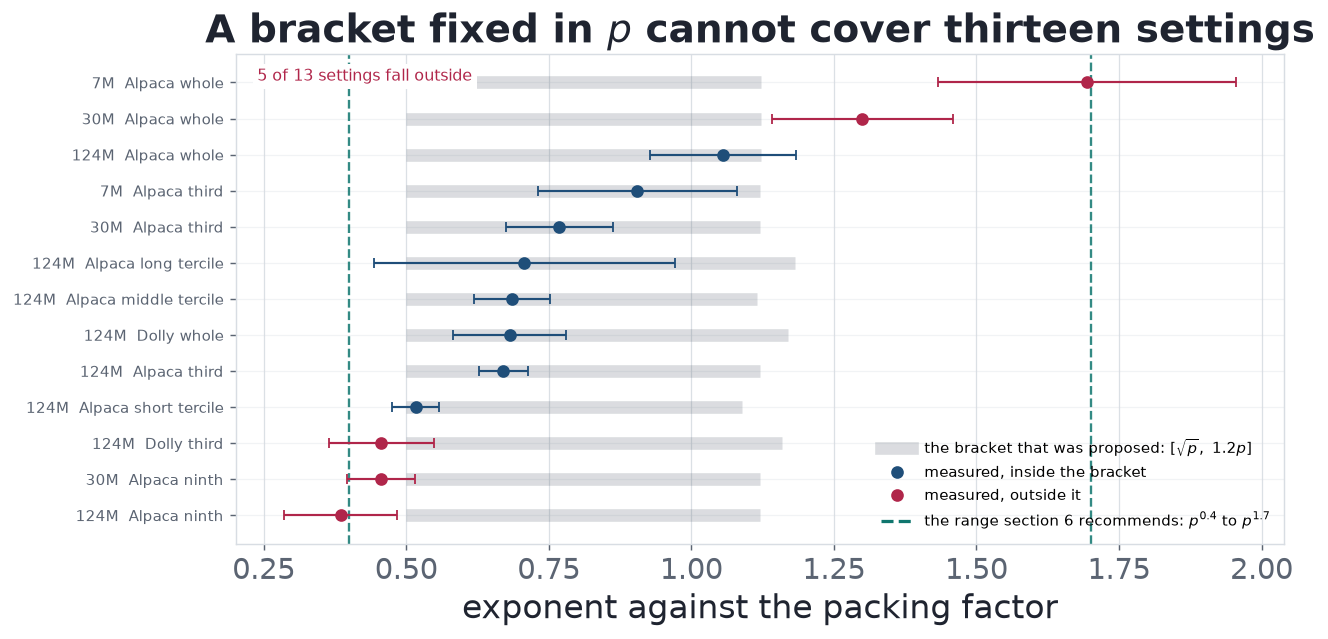
\includegraphics[width=\linewidth]{figures/10-lr-scaling-bracket.png}
\caption{Every one of the thirteen settings against the bracket an earlier draft proposed. In exponent terms that bracket is 0.5 at the floor and log(1.2p)/log(p) at the ceiling (about 1.12 to 1.17 over the packing factors here), drawn as the grey band. Five settings fall outside it, and not at random: the three below the floor are the three smallest-scale settings, and the two above the ceiling are the two smaller models on the largest corpus. The dashed verticals are the range this section recommends instead. Error bars are the seed bound of \S{}4.5.}
\end{figure}

What the measurements support instead is a range. Across all thirteen settings the exponent runs from \textbf{0.412 to 1.695}, so the packed optimum sits somewhere in

[ lr\_pad \emph{ p\textasciicircum{}0.4,  lr\_pad } p\textasciicircum{}1.7 ]

a span of \texttt{p\textasciicircum{}1.3}: a factor of 4.0 at Dolly's packing ratio, 7.0 at Alpaca's and 14.5 at the widest one here. Three points at 1.6x spacing cover the first, and six the last.

That spacing is coarse on purpose, and how coarse it can be is measurable rather than a matter of taste. Near its minimum the loss-versus-log(lr) curve is locally quadratic (the same assumption \S{}3.3's estimator makes), and its curvature is strikingly consistent across everything measured here: 0.027 to 0.066 nats per log(lr) squared, over three model sizes, both arms and a 13x range of optimal learning rate. Landing one 1.6x step off the bottom therefore costs between 0.006 and 0.015 nats, against the 0.050 to 0.172 that inheriting costs (\S{}4.7). A sweep this coarse captures 84\% to 97\% of what retuning is worth, and the residual is smaller than this study's seed spread.

The practical reading is that precision is cheap and being in the right neighbourhood is not. Missing the optimum by a factor of 1.6 is nearly free; missing it by the factor of 1.7 to 12.7 that inheriting implies is not. \texttt{scripts/\allowbreak{}analyze\_\allowbreak{}optimum\_\allowbreak{}sharpness.py} reports the curvatures. That is a real sweep rather than a nudge, and it is the honest cost of the fact that no exponent generalises: we can offer where to look, not where the answer is. Two things narrow it in practice, and both were registered or replicated rather than fitted. A larger run pushes the exponent up, so production-scale training should look in the upper half; a smaller model pushes it up too, though only the 17x span establishes that (\S{}4.7). What does \emph{not} narrow it is how well the base model was pretrained, which moves both optima together and the exponent not at all (\S{}4.7.1), so a practitioner cannot transfer our \texttt{lr\_\allowbreak{}pad}, only the distance from theirs. If the minimum lands on an edge, extend and re-run: an unbracketed minimum is not a measurement (\S{}3.3).

What no candidate inside that range does is as badly as inheriting, which assumes an exponent of zero and is wrong by factors of 1.7 to 12.7 across these settings.

\textbf{Do not tune this at a matched step count.} The recipe above is for a matched data budget, which is what a practitioner turning packing on actually has. At a matched step count the packed arm consumes \texttt{p} times the data and, on corpora this size, runs enough epochs that the apparent optimum is set by which rate overfits least (Appendix B). That cell answers a different question and should not be used to pick a production learning rate.

\textbf{Report which comparison you ran.} The reason the literature can assert that the learning rate need not move, and the reason our own earlier reading of these corpora (Appendix A) called the shift linear batch scaling, is the same: at a fixed data budget packing moves batch size and step count together, and a single ratio measured across that diagonal is consistent with rules that disagree everywhere else. Any claim about learning rate under packing needs to say whether the step count was held fixed, and any factorial that holds it fixed needs to say how many epochs each arm ran.

\section{Conclusion}

We set out to check a piece of standard advice, that packing is an efficiency change and the learning rate can be inherited through it, and it does not survive contact with a sweep. The optimum moves by 1.7x to 12.7x across the settings measured here, inheriting gives back most of what packing offers, and on several settings a packed run at the inherited rate does not beat the padded run it inherited from.

What packing is doing is settled, as far as this evidence goes. Assembling the same batch by padding instead (matched on supervised tokens, examples and data seen, at several times the forward-pass cost) reaches the same optimum, so the optimum is set by what a step contains and not by how it is laid out. That also explains why Krell et al.'s original recipe, which shrinks the batch by the packing factor, needs no learning-rate change: it is the practice of packing to make the step \emph{bigger} that is exposed.

How much the optimum moves is not settled, and we think it is not settleable in the form the question is usually asked. There is no exponent to report: it runs from 0.41 to 1.70, it rises with the scale of the run on two corpora and three model sizes, it rises as the model shrinks, and it is indifferent to how well the base model was pretrained: across a doubling of the pretraining budget at fixed size, and across a 4.6-fold change in perplexity at fixed size. A bracket we proposed in an earlier draft of this paper fails on five of thirteen settings and is retracted here rather than quietly dropped.

What would move this forward is not more seeds. It is model sizes above 124M, corpora drawn independently rather than sliced from two, and batches near the scales where production fine-tuning actually runs. The fourth item on that list was a metric other than same-corpus held-out loss, and \S{}4.3 now carries one: scored on a corpus it was not tuned on, the retuned packed run loses to the inherited one by 0.087 nats, having beaten it by 0.050 on the corpus it was tuned on. That does not move the optima (where the minimum of same-corpus loss sits is what this paper measures), but it means the \emph{worth} of retuning is a statement about one distribution, and a reader who wants it to be more than that should measure their own. Until then the honest recipe is the sweep in \S{}6: three to six points, spanning \texttt{p\textasciicircum{}0.4} to \texttt{p\textasciicircum{}1.7}, and no inherited rate.

\section*{References}
\begingroup
\small
\setlength{\parindent}{0pt}

\hangindent=1.5em\hangafter=1 Goyal, Doll\'ar, Girshick, Noordhuis, Wesolowski, Kyrola, Tulloch, Jia, He (2017). \emph{Accurate, Large Minibatch SGD: Training ImageNet in 1 Hour.} arXiv:1706.02677\par

\hangindent=1.5em\hangafter=1 Krell, Kosec, Perez, Fitzgibbon (2021). \emph{Efficient Sequence Packing without Cross-contamination: Accelerating Large Language Models without Impacting Performance.} arXiv:2107.02027\par

\hangindent=1.5em\hangafter=1 Li, Zhao, Zhang, Sun, Wu, Jiao, Wang, Liu, Fang, Xue, Tao, Cui, Wang (2024). \emph{Surge Phenomenon in Optimal Learning Rate and Batch Size Scaling.} NeurIPS 2024. arXiv:2405.14578\par

\hangindent=1.5em\hangafter=1 Malladi, Lyu, Panigrahi, Arora (2022). \emph{On the SDEs and Scaling Rules for Adaptive Gradient Algorithms.} arXiv:2205.10287\par

\hangindent=1.5em\hangafter=1 McCandlish, Kaplan, Amodei, OpenAI Dota Team (2018). \emph{An Empirical Model of Large-Batch Training.} arXiv:1812.06162\par

\hangindent=1.5em\hangafter=1 Shallue, Lee, Antognini, Sohl-Dickstein, Frostig, Dahl (2019). \emph{Measuring the Effects of Data Parallelism on Neural Network Training.} JMLR 20(112):1-49. arXiv:1811.03600\par

\hangindent=1.5em\hangafter=1 Smith, Kindermans, Ying, Le (2018). \emph{Don't Decay the Learning Rate, Increase the Batch Size.} ICLR 2018. arXiv:1711.00489\par

\hangindent=1.5em\hangafter=1 Wang, Aitchison (2024). \emph{Batch size invariant Adam.} NeurIPS 2024. arXiv:2402.18824\par

\hangindent=1.5em\hangafter=1 Wang, Wang, Wang, Li, Hovy, Guo (2025). \emph{Packing Analysis: Packing Is More Appropriate for Large Models or Datasets in Supervised Fine-tuning.} Findings of ACL 2025, 2025.findings-acl.256. arXiv:2410.08081\par

\emph{(Author lists, titles and venues checked against the arXiv, JMLR and ACL Anthology records. The three claims attributed to Krell et al. in section 2 (the advice against learning-rate scaling, the LAMB heuristic, and reducing the computational batch size by the packing factor) are their section 3.3. The three claims attributed to Wang et al. (the quoted sentence, the 1e-5 held across both arms, and the batch-size-and-learning-rate comparison) are their section 5.3 and their training-details table, checked against arXiv:2410.08081v3 on 2026-08-30. The linear-scaling claim attributed to Wang and Aitchison, including their remark that the linear and square-root rules are "not a contradiction: both are correct in their respective setups", is their section 1; the square-root camp they place it against is Granziol et al. (2022), Malladi et al. (2022) and Hilton et al. (2022), of which we cite the second.)}

\endgroup

\section*{Appendix}

Material the argument rests on but does not need in line: the check that the harness reproduces the measurement it replaces, the methodological trap that shaped the design, the seed accounting behind every optimum, and how to re-run all of it.

\appendix
\section{The harness reproduces the original measurement}

Nine of the grid's learning rates were run in this project before, under the hand-written configs that preceded this sweep harness. Eight reproduce to four decimals and the ninth differs by 0.0001:

\begin{center}
\small
\setbox0=\hbox{%
\begin{tabular}{lrrrrr}
\toprule
cell & 2.0e-5 & 3.0e-5 & 6.0e-5 & 9.0e-5 & 1.5e-4 \\
\midrule
packed, 350 steps, prior & 2.0912 & 2.0678 & 2.0352 & 2.0217 & 2.0175 \\
packed, 350 steps, here & 2.0911 & 2.0678 & 2.0352 & 2.0217 & 2.0175 \\
padded, 1,600 steps, prior & 2.0745 & 2.0720 & 2.0973 & --- & --- \\
padded, 1,600 steps, here & 2.0745 & 2.0720 & 2.0973 & --- & --- \\
\bottomrule
\end{tabular}}
\ifdim\wd0>\linewidth\resizebox{\linewidth}{!}{\usebox0}\else\usebox0\fi
\end{center}

The sweep is therefore measuring the same quantity the original tables did, on generated configs, and the two new cells are directly comparable to the two old ones.

\section{The overfitting trap, and the metric it biases}

Neither factorial decomposes cleanly. Read Alpaca's batch effect at 1,600 steps rather than 350 and it is \textbf{0.83x} (the optimum moves the wrong way), and Dolly's at 430 steps is \textbf{0.64x}. Both anomalies live in the same place: the packed cell at the long step count, which runs 4.50 epochs on Alpaca and 2.92 on Dolly.

Those cells overfit. Alpaca's best validation loss arrives at step 684--1368 rather than at the end, and it arrives earlier the higher the learning rate, so the apparent optimum is set by which rate overfits least by the final step. Scored on best-during-run instead of endpoint, Alpaca's packed 1,600 optimum rises from 2.25e-5 to 3.61e-5 (both seed 1337, so that the two metrics are compared on one curve), and the anomaly shrinks without disappearing.

How far this reaches is worth measuring rather than asserting, because the choice of metric is otherwise invisible. Scoring every cell in the study both ways (17 cells at seed 1337, across five corpora, both packing modes, and the wide-batch control):

\begin{center}
\small
\setbox0=\hbox{%
\begin{tabular}{lrl}
\toprule
epochs the cell runs & cells & optimum under best-checkpoint scoring \\
\midrule
0.22 to 1.01 & 15 & unchanged, \textbf{1.00x in every one} \\
2.92 (Dolly packed, 430 steps) & 1 & \textbf{1.29x} \\
4.50 (Alpaca packed, 1,600 steps) & 1 & \textbf{1.60x} \\
\bottomrule
\end{tabular}}
\ifdim\wd0>\linewidth\resizebox{\linewidth}{!}{\usebox0}\else\usebox0\fi
\end{center}

The threshold is sharp, and nothing in this study falls between 1.01 and 2.92 epochs to soften it. In all fifteen cells at or under one epoch no run peaks before its final step, so the two metrics are not merely close: they are the same measurement, and return the same optimum to the digit. At 1.01 epochs runs do begin to peak early, but by 0.0005 nats, and the optimum still does not move. Only past about three epochs does the choice of metric change the answer. How far past matters: the 4.50-epoch cell's 1.60x exceeds every seed spread measured anywhere in this study, including the 1.37x of Appendix C, while the 2.92-epoch cell's 1.29x exceeds the worst spread among the 124M cells this table covers (1.25x) but not that 1.37x. So the first is a metric effect larger than the noise on any cell here and the second is at the edge of it, which is one more reason to keep both out of the headline rather than to correct them.

The mechanism is specific, and it is why the bias has a direction rather than being noise. The endpoint penalty (how much a run gives back after its own best checkpoint) rises monotonically with the learning rate, from 0.0000 to 0.4269 nats across Alpaca's packed 1,600-step grid and from 0.0000 to 0.2962 across Dolly's packed 430-step grid. The endpoint metric therefore charges the higher learning rates for overfitting they did \emph{after} already passing their own minimum, and the argmin moves down for a reason that has nothing to do with step size.

The general form is worth stating for anyone running this design: \textbf{at a matched step count, an arm that runs many epochs reports an optimum depressed by overfitting, and a factorial that ignores this attributes the depression to whatever else that arm varied.} \texttt{scripts/\allowbreak{}analyze\_\allowbreak{}lr\_\allowbreak{}scaling.py} excludes cells past 1.5 epochs from its headline for this reason, and \texttt{scripts/\allowbreak{}analyze\_\allowbreak{}metric\_\allowbreak{}bias.py} reproduces the table above.

\section{Status of the evidence}

Alpaca's four optima were re-run at seeds 1338 and 1339 on the three learning rates bracketing each. Solving each seed's curve separately, as 3.1 requires, the optima are 5.00e-5, 2.81e-5, 1.37e-4 and 2.35e-5, with max/min spreads across seeds of 1.13x, 1.17x, 1.11x and 1.08x. The first three aggregate all three seeds. The packed 1,600-step cell aggregates two: at seed 1339 its minimum falls on the edge of the three points that were run for replication, so that curve brackets nothing and we drop it rather than extrapolate from it. That cell is excluded from the headline in any case (Appendix B). None of the effects in \S{}4.2 or \S{}4.3 changes sign or materially in magnitude against the single-seed values.

Dolly's three cells that are not overfitting-contaminated were replicated the same way, with spreads of 1.08x, 1.11x and 1.03x. That spread is the yardstick \S{}4.2 is measured against: it is what makes a 1.28x miss a failed prediction rather than a noisy one.

The six subsets of \S{}4.5 and \S{}4.6 were replicated the same way, and every exponent quoted from them carries the resulting bound. Worst-cell spreads run 1.06x to 1.25x: Alpaca's short, middle and long terciles at 1.08x, 1.20x and 1.25x, its random ninth and third at 1.19x and 1.06x, and Dolly's third at 1.10x. Every cell brackets its optimum at all three seeds.

That last sentence is newer than the rest of this appendix. The middle tercile and the random ninth stood at two seeds each for most of this study, because in each a third seed put its minimum on the edge of the replicated points and the rule elsewhere is to drop such a curve rather than extrapolate from it. Both have now been extended instead, one point each, and both bracket. The reason for extending is the one \S{}4.7.2's padded cell already established: dropping is only neutral when the drop is not systematic, and neither of these was. The ninth's dropped seed sat \emph{above} its window and the tercile's \emph{below} it, so dropping them biased one exponent down and the other up. Alpaca's packed 1,600-step cell was extended at the same time and now brackets too, which leaves \textbf{no curve anywhere in this paper resting on fewer than three seeds, and none dropped}.

It moved two numbers, both inside their own bounds and both with the bound roughly doubled, because the curve that had been dropped was in each case the one furthest from the other two. The middle tercile went from 0.686 $\pm$ 0.067 to \textbf{0.651 $\pm$ 0.133} and the random ninth from 0.385 $\pm$ 0.100 to \textbf{0.412 $\pm$ 0.136}. The ninth is one end of the range \S{}6 recommends, so the paper's headline span is now 0.412 to 1.695 rather than 0.385 to 1.695, and the first step of \S{}4.6's scale series clears its combined bound by 1.8x where it previously cleared it by 2.6x. Nothing changes sign and no conclusion turns, but the scale series is measurably weaker at its small end than the earlier version of this appendix claimed, and that is the direction an honest replication is expected to move in.

Two earlier replications had already changed a number this paper reported, and both are recorded where they were claimed. The random third moved from 0.685 to 0.670, \emph{toward} the value registered for it, not away. The random ninth moved from 0.316 to 0.385, which dissolved the straight line \S{}4.6 had already flagged as too regular to be real, and has now moved again to 0.412 for the reason above. Neither reverses a conclusion; the second retires an artefact, and \S{}4.6 reports it as the caution being borne out rather than quietly restating the table.

The loss tables in \S{}4.1 and the inherit-versus-retune table in \S{}4.3 are seed 1337 throughout. They have to be: a seed changes which examples are held out, so losses are comparable down a column within one seed and not across seeds. Only the optima are aggregated across seeds, and only after each seed is solved on its own curve. One consequence is worth stating plainly: the replication seeds were run on the points bracketing each optimum, which does not include the inherited rate, so \S{}4.3's comparison has no cross-seed check behind it. That is the reason \S{}4.3 leans on the inherit-to-retune distance rather than on the sign of the inherit-to-padding difference.

The three cells of \S{}4.7 and \S{}4.7.1 that are not at 124M were replicated the same way, and here the replication is cleaner than at 124M: all fourteen cells across the 30M, 7M and matched-budget-30M ledgers bracket their optimum at all three seeds, with none dropped. Their spreads run 1.06x to 1.37x: 30M's six cells at 1.06x to 1.23x, the matched-budget 30M's four at 1.09x to 1.17x, and 7M's four at 1.20x to 1.37x. The 7M packed 350-step cell's 1.37x is the widest spread among them, which is why \S{}4.7's bounds are widest at 7M and why the model-size claim is stated only at the 17x span: the smallest model is also the noisiest, and the bounds carry that through rather than around it.

Two cells there were bracketed only after the fact, and the sequence is worth recording because it is the same trap \S{}3.3 warns about. On the 7M model the replication seeds were first run on the three learning rates bracketing seed 1337's optimum, and on three of the eight cells a replication seed put its minimum on the \emph{edge} of that window, twice at the top and once at the bottom. Dropping those curves, as we do elsewhere, would have left the 7M random third resting on a single seed with a $\pm$0.006 bound that reflected nothing. But the drops were not symmetric (two of the three fell above their window), so dropping them would have biased the surviving estimate downward rather than merely widening it. We extended the window instead, at four more runs, and all three then bracketed. The bound on that cell went from $\pm$0.006 to $\pm$0.174, which is the honest number and is nearly forty times larger.

The two ledgers added last (\S{}4.7.1's 7M matched-budget control and \S{}4.7.2's quality control) were replicated the same way, and needed the window extended twice more. All four cells of the 7M matched-budget ledger now bracket at three seeds, with spreads of 1.15x, 1.23x, 1.25x and 1.62x; the last of these, its padded whole-corpus cell, is the widest spread anywhere in this study and is why \S{}4.7.1 calls that pair the weakest of its four even though it agrees with them. Both of \S{}4.7.2's cells bracket at three seeds, at 1.22x and 1.26x.

Three curves across those two ledgers first put their minimum on the edge of the replicated window, two at the top and one at the bottom, and in each case dropping the curve, which is the rule everywhere above, would have moved the surviving estimate in a known direction rather than merely widening it. The window was extended instead, as it was for the 7M random third: six more runs. The case worth stating is \S{}4.7.2's, because it ran against the hypothesis being tested. Its padded cell's unbracketed seed sat above the other two, so dropping it would have pulled that arm down and pushed the exponent \emph{up}, toward the quality reading its registered prediction argued against. On two seeds that exponent read 0.946; on three it reads 0.906. Both confirm H1 and the difference is well inside the bound either way, but the drop would not have been neutral, and reporting the two-seed number as though it were would have been wrong.

Everything in \S{}4.1 through \S{}4.6 is one model size (124M) on two corpora at one window length; \S{}4.7 adds two more sizes, \S{}4.7.1 a second pretraining budget at two of them, and \S{}4.7.2 a base model matched on quality rather than on size, all of them on Alpaca only.

\section{Reproducibility}

Every number in this paper comes from one of nine ledgers, one per base model, each a row per run: dataset, cell, learning rate, seed, final and best validation loss, the step the best arrived at, and wall time. The sweep is resumable and skips rows already present, so each file is both the output and the ledger.

\begin{center}
\small
\setbox0=\hbox{%
\begin{tabular}{lll}
\toprule
ledger & base model & sections \\
\midrule
\texttt{results/\allowbreak{}lr\_\allowbreak{}scaling\_\allowbreak{}sweep.csv} & 124M & \S{}4.1--\S{}4.6 \\
\texttt{results/\allowbreak{}lr\_\allowbreak{}scaling\_\allowbreak{}small.csv} & 30M, 39.4 tokens/param & \S{}4.7 \\
\texttt{results/\allowbreak{}lr\_\allowbreak{}scaling\_\allowbreak{}mini.csv} & 7M, 39.5 tokens/param & \S{}4.7 \\
\texttt{results/\allowbreak{}lr\_\allowbreak{}scaling\_\allowbreak{}small9k.csv} & 30M, 19.7 tokens/param & \S{}4.7.1 \\
\texttt{results/\allowbreak{}lr\_\allowbreak{}scaling\_\allowbreak{}mini2k.csv} & 7M, 18.0 tokens/param & \S{}4.7.1 \\
\texttt{results/\allowbreak{}lr\_\allowbreak{}scaling\_\allowbreak{}quality.csv} & 124M, perplexity 107.0 & \S{}4.7.2 \\
\texttt{results/\allowbreak{}lr\_\allowbreak{}scaling\_\allowbreak{}quality2500.csv} & 124M, perplexity 39.4 & \S{}4.7.2 \\
\texttt{results/\allowbreak{}lr\_\allowbreak{}scaling\_\allowbreak{}downstream.csv} & 124M, \S{}4.3's kept checkpoints & \S{}4.3 \\
\texttt{results/\allowbreak{}lr\_\allowbreak{}scaling\_\allowbreak{}ckpt.csv} & 124M, grid extension & Appendix E \\
\bottomrule
\end{tabular}}
\ifdim\wd0>\linewidth\resizebox{\linewidth}{!}{\usebox0}\else\usebox0\fi
\end{center}

They are separate files rather than one file with a model column because they were not always: \texttt{run\_\allowbreak{}id} is (dataset, cell, learning rate, seed) and says nothing about the base model, so the first 30M sweep appended its curves to the 124M runs' log files and its \texttt{best\_\allowbreak{}val\_\allowbreak{}loss} picked up 124M minima. Logs, configs and checkpoints are now namespaced per ledger, and that ledger was discarded and re-run.

\begingroup\small
\begin{verbatim}
# the two factorials (28 runs each, seed 1337)
python scripts/sweep_lr_packing.py --gpus 0 1
python scripts/sweep_lr_packing.py --dataset dolly --gpus 0 1

# seed replication, on the three learning rates bracketing each optimum
python scripts/sweep_lr_packing.py --seeds 1338 1339 --lrs <three points>

# packing factors in supervised tokens per step, measured not assumed
python scripts/benchmark_packing.py --data data/sft/alpaca.jsonl
python scripts/benchmark_packing.py --data data/sft/dolly.jsonl

# the wide-batch control of 4.4: an unpacked step with the packed step's batch
python scripts/sweep_lr_packing.py --cells wide_350 --gpus 0 1
python scripts/sweep_lr_packing.py --dataset dolly --cells wide_136 --gpus 0 1

# the other model sizes of 4.7, and the matched-budget checkpoint of 4.7.1.
# --model-config and --init-from are what keep a ledger to one base model.
python scripts/sweep_lr_packing.py --dataset alpaca_third \
    --model-config configs/model/mini.yaml \
    --init-from checkpoints/mini/step_4400.pt \
    --results results/lr_scaling_mini.csv --gpus 0 1
python scripts/sweep_lr_packing.py --dataset alpaca \
    --model-config configs/model/small.yaml \
    --init-from checkpoints/small/step_9000.pt \
    --results results/lr_scaling_small9k.csv --gpus 0 1

# the tables in 4.2, the optima, and the headline ratios in 4.3
python scripts/analyze_lr_scaling.py --dataset alpaca
python scripts/analyze_lr_scaling.py --dataset dolly

# every exponent in 4.5 through 4.7.1, across all seven ledgers, as one table
python scripts/export_exponents.py          # -> results/exponents.csv

# the fp16 claim in section 5, over every run log rather than a sample
python scripts/check_numerical_stability.py

# Appendix G: every conclusion under two other normalizations of the shift
python scripts/check_normalization_robustness.py

# how sharp the optima are, which is what section 6's sweep spacing rests on
python scripts/analyze_optimum_sharpness.py

# the figures in 4.1, 4.4 and 4.6
python scripts/plot_results.py --only lr-scaling
\end{verbatim}
\endgroup

\texttt{scripts/\allowbreak{}analyze\_\allowbreak{}metric\_\allowbreak{}bias.py} reports the endpoint-versus-best-checkpoint comparison, and \texttt{scripts/\allowbreak{}analyze\_\allowbreak{}packing\_\allowbreak{}series.py} the packing-ratio series.

\texttt{scripts/\allowbreak{}analyze\_\allowbreak{}lr\_\allowbreak{}scaling.py} is the single place the optima are solved: it fits the parabola of 3.3, keeps each seed's curve separate for the reason in 3.1, drops a seed whose curve brackets no minimum, and excludes cells past 1.5 epochs from the headline for the reason in Appendix B. The tables in \S{}4.1 and the ratios in \S{}4.2 are its output rather than transcriptions of it.

Hardware is a single RTX 2080 Ti per run, and the whole grid is about 70 GPU-hours (measured across the 672 runs that recorded wall time; 2 rows carry no wall time, having been harvested from earlier runs of the same configs). One caveat for anyone reproducing the schedule estimate rather than the science: the second card in this machine thermally throttles under sustained load and takes about 2.5x as long per step, which the sweep's planner accounts for and a naive divide-by-GPU-count does not.

\section{The full loss grids}

Final validation loss at every learning rate in the grid, seed 1337, for the two whole corpora. Section 4.1 reports the optima these are interpolated from; the grids themselves are here because what matters in the text is where each curve turns, not the fifty-six numbers it turns among.

\textbf{Alpaca.} One packed epoch is 350 steps and one padded epoch is 1,600.

\begin{center}
\small
\setbox0=\hbox{%
\begin{tabular}{lrrrrrrr}
\toprule
cell & 1e-5 & 2e-5 & 3e-5 & 6e-5 & 9e-5 & 1.5e-4 & 2.5e-4 \\
\midrule
padded, 350 & 2.1885 & 2.1539 & 2.1397 & \textbf{2.1338} & 2.1466 & 2.1907 & 2.2770 \\
padded, 1,600 & 2.0973 & 2.0745 & \textbf{2.0720} & 2.0973 & 2.1335 & 2.2091 & 2.3149 \\
packed, 350 & 2.1353 & 2.0911 & 2.0678 & 2.0352 & 2.0217 & \textbf{2.0175} & 2.0319 \\
packed, 1,600 & 2.0421 & \textbf{2.0171} & 2.0197 & 2.0845 & 2.1789 & 2.3616 & 2.5703 \\
\bottomrule
\end{tabular}}
\ifdim\wd0>\linewidth\resizebox{\linewidth}{!}{\usebox0}\else\usebox0\fi
\end{center}

The packed 1,600-step cell ran at 2.5e-4 only after the rest of the grid was complete; its absence could not have moved that cell's optimum, which sits at the opposite end of the grid.

\textbf{Dolly.} One packed epoch is 136 steps and one padded epoch is 430.

\begin{center}
\small
\setbox0=\hbox{%
\begin{tabular}{lrrrrrrr}
\toprule
cell & 1e-5 & 2e-5 & 3e-5 & 6e-5 & 9e-5 & 1.5e-4 & 2.5e-4 \\
\midrule
padded, 136 & 2.8277 & 2.8043 & 2.7931 & \textbf{2.7868} & 2.7978 & 2.8372 & 2.9178 \\
padded, 430 & 2.7801 & 2.7588 & \textbf{2.7517} & 2.7567 & 2.7765 & 2.8253 & 2.9180 \\
packed, 136 & 2.8071 & 2.7799 & 2.7662 & 2.7505 & \textbf{2.7484} & 2.7604 & 2.7973 \\
packed, 430 & 2.7596 & \textbf{2.7429} & 2.7430 & 2.7824 & 2.8433 & 2.9742 & 3.1525 \\
\bottomrule
\end{tabular}}
\ifdim\wd0>\linewidth\resizebox{\linewidth}{!}{\usebox0}\else\usebox0\fi
\end{center}

Every optimum in both grids is bracketed (an interior minimum with a rise on both sides), including the packed short-step cell, which that earlier sweep took only as far as 1.5e-4 and could not bracket.

\section{Every comparison in one table}

The paper's central claim is that the exponent has no single value, and that claim is spread across \S{}4.5 to \S{}4.7.2 a few settings at a time. This is all of it at once, so that the spread can be read rather than taken on the text's word.

Every row is a matched-budget comparison: one epoch padded against one epoch packed, each arm solved for its own optimum on its own seed's curve, aggregated across seeds as \S{}3.1 requires. \texttt{p} is the ratio of supervised tokens per optimizer step, measured rather than assumed. The exponent is \texttt{log(shift) /\allowbreak{} log(p)}, and the bound carries both cells' max/min seed ranges through that ratio, so it is a range and not a standard error (\S{}4.5).

\begin{center}
\small
\setbox0=\hbox{%
\begin{tabular}{llrrrrrrr}
\toprule
base model & corpus & examples & \texttt{p} & lr* padded & lr* packed & shift & exponent & seeds \\
\midrule
124M & Alpaca, random ninth & 5,652 & 4.53x & 5.83e-05 & 1.09e-04 & 1.86x & \textbf{0.412 $\pm$ 0.136} & 3 \\
124M & Alpaca, short tercile & 16,956 & 7.84x & 4.80e-05 & 1.39e-04 & 2.90x & \textbf{0.517 $\pm$ 0.042} & 3 \\
124M & Alpaca, middle tercile & 16,956 & 4.87x & 4.48e-05 & 1.26e-04 & 2.80x & \textbf{0.651 $\pm$ 0.133} & 3 \\
124M & Alpaca, long tercile & 16,956 & 2.73x & 6.73e-05 & 1.37e-04 & 2.03x & \textbf{0.707 $\pm$ 0.265} & 3 \\
124M & Alpaca, random third & 16,956 & 4.51x & 4.59e-05 & 1.26e-04 & 2.74x & \textbf{0.670 $\pm$ 0.043} & 3 \\
124M & Alpaca, whole & 50,868 & 4.47x & 2.81e-05 & 1.37e-04 & 4.86x & \textbf{1.055 $\pm$ 0.128} & 3 \\
124M & Dolly, random third & 4,585 & 3.14x & 4.66e-05 & 7.87e-05 & 1.69x & \textbf{0.456 $\pm$ 0.092} & 3 \\
124M & Dolly, whole & 13,756 & 2.92x & 3.78e-05 & 7.84e-05 & 2.07x & \textbf{0.681 $\pm$ 0.099} & 3 \\
30M & Alpaca, random ninth & 5,652 & 4.53x & 8.23e-05 & 1.64e-04 & 1.99x & \textbf{0.456 $\pm$ 0.059} & 3 \\
30M & Alpaca, random third & 16,956 & 4.51x & 6.31e-05 & 2.01e-04 & 3.18x & \textbf{0.768 $\pm$ 0.094} & 3 \\
30M & Alpaca, whole & 50,868 & 4.47x & 3.50e-05 & 2.45e-04 & 7.01x & \textbf{1.300 $\pm$ 0.159} & 3 \\
7M & Alpaca, random third & 16,956 & 4.51x & 1.89e-04 & 7.39e-04 & 3.91x & \textbf{0.905 $\pm$ 0.174} & 3 \\
7M & Alpaca, whole & 50,868 & 4.47x & 1.19e-04 & 1.51e-03 & 12.66x & \textbf{1.695 $\pm$ 0.261} & 3 \\
30M @ 19.7 tok/param & Alpaca, random third & 16,956 & 4.51x & 9.19e-05 & 3.01e-04 & 3.27x & \textbf{0.787 $\pm$ 0.100} & 3 \\
30M @ 19.7 tok/param & Alpaca, whole & 50,868 & 4.47x & 5.06e-05 & 3.56e-04 & 7.03x & \textbf{1.302 $\pm$ 0.119} & 3 \\
7M @ 18.0 tok/param & Alpaca, random third & 16,956 & 4.51x & 2.73e-04 & 1.04e-03 & 3.80x & \textbf{0.886 $\pm$ 0.201} & 3 \\
7M @ 18.0 tok/param & Alpaca, whole & 50,868 & 4.47x & 2.19e-04 & 2.38e-03 & 10.85x & \textbf{1.592 $\pm$ 0.333} & 3 \\
124M @ perplexity 39.4 & Alpaca, whole & 50,868 & 4.47x & 5.22e-05 & 2.85e-04 & 5.46x & \textbf{1.133 $\pm$ 0.107} & 3 \\
124M @ perplexity 107 & Alpaca, whole & 50,868 & 4.47x & 1.12e-04 & 4.36e-04 & 3.88x & \textbf{0.906 $\pm$ 0.204} & 3 \\
\bottomrule
\end{tabular}}
\ifdim\wd0>\linewidth\resizebox{\linewidth}{!}{\usebox0}\else\usebox0\fi
\end{center}

Read down a group and the scale dependence of \S{}4.6 is the trend; read the same corpus across groups and the model-size dependence of \S{}4.7 is the trend. The last three groups are not further model sizes but controls. The two \texttt{tok/\allowbreak{}param} groups are \S{}4.7.1's, the same 30M and 7M architectures pretrained on about half the token budget: their exponents sit on top of the fully pretrained ones (the four differences are 0.019, 0.002, 0.019 and 0.103, every one inside its bound), while their learning rates sit 1.4x to 1.8x above them, in both arms. The final row is \S{}4.7.2's, 124M weights from an early pretraining checkpoint at the 7M model's perplexity: its learning rates are three to four times the fully pretrained 124M model's, and its exponent stays with 124M's own rather than moving to 7M's.

The table is regenerated from \texttt{results/\allowbreak{}exponents.csv} by \texttt{scripts/\allowbreak{}update\_\allowbreak{}paper\_\allowbreak{}counts.py} rather than transcribed, so it cannot drift from the estimator in \texttt{scripts/\allowbreak{}analyze\_\allowbreak{}lr\_\allowbreak{}scaling.py} that produced it.

\section{Is it the data, or is it the normalization?}

\S{}3.3 flags that the exponent is a choice of summary. This appendix measures how much each conclusion depends on it, by recomputing all three under two alternatives:

\begin{center}
\small
\setbox0=\hbox{%
\begin{tabular}{lll}
\toprule
 & statistic & what it assumes \\
\midrule
\texttt{power} & \texttt{log(shift) /\allowbreak{} log(p)} & the shift is a power of \texttt{p}, what we report \\
\texttt{linear} & \texttt{(shift - 1) /\allowbreak{} (p - 1)} & the shift is linear in \texttt{p} \\
\texttt{sqrtrel} & \texttt{shift /\allowbreak{} sqrt(p)} & the residual against the square-root rule \\
\bottomrule
\end{tabular}}
\ifdim\wd0>\linewidth\resizebox{\linewidth}{!}{\usebox0}\else\usebox0\fi
\end{center}

Seed bounds are propagated exactly rather than by a delta approximation: the ledger's bound is converted back to the multiplicative factor it implies on the shift, each statistic is evaluated at both ends, and the half-width of that interval is taken. The intervals are asymmetric under the two non-log forms, which is why the approximation is avoided.

\begin{center}
\small
\setbox0=\hbox{%
\begin{tabular}{lrrrl}
\toprule
conclusion & \texttt{power} & \texttt{linear} & \texttt{sqrtrel} & verdict \\
\midrule
Scale moves it (whole vs third, 124M) & 2.85x & 2.24x & 2.23x & \textbf{clears under all three} \\
The tercile ratio trend is unsupported & 0.71x & \textbf{1.01x} & 0.57x & holds, but only just under \texttt{linear} \\
Alpaca third and Dolly whole agree & 0.10x & 0.50x & 0.51x & \textbf{agree under all three} \\
Alpaca ninth and Dolly third agree & 0.27x & 0.55x & 0.37x & \textbf{agree under all three} \\
\bottomrule
\end{tabular}}
\ifdim\wd0>\linewidth\resizebox{\linewidth}{!}{\usebox0}\else\usebox0\fi
\end{center}

Each number is the gap between the two settings as a multiple of their combined seed bound, under that normalization.

The central claim is not an artefact of the summary. Scale clears its bound under every normalization tried, which is what \S{}3.3 predicts: that comparison holds \texttt{p} to within 1\%, so it is really a statement that the raw shift moves from 1.86x to 2.74x to 4.86x, and no monotone rescaling of a ratio can undo that. The same argument covers the model-size series of \S{}4.7, whose \texttt{p} is identical across the three sizes to four significant figures.

The one that is exposed is the tercile null, and it is exposed in the direction of the retraction rather than against it. Under \texttt{power} the three terciles span 0.71x their noise and under \texttt{sqrtrel} 0.57x, and under \texttt{sqrtrel} they are not even monotone; under \texttt{linear} the spread is 1.01x its noise, equal to it, which is not evidence of a trend but is close enough that we say so rather than lean on the 0.71x. \S{}4.5 reports the packing-ratio trend as unsupported, and that verdict is the same under all three, though not equally comfortably.

The cross-corpus agreement survives, but it is tightest under the normalization we report. Alpaca's third and Dolly agree to 0.10x of their bound as exponents and to 0.50x and 0.51x under the alternatives. All three are agreement within noise, so the conclusion of \S{}4.6 stands whichever is used, but the striking closeness of the exponents is partly a property of the exponent. Read the other way this is mild evidence \emph{for} the power-law summary (a normalization that removes \texttt{p}-dependence should make settings at matched scale and different \texttt{p} agree, and this one does so better than the alternatives), but on two pairs that is a remark and not a result.

\textbf{What none of this addresses.} Every form here is a one-parameter rescaling of a ratio. If the optimum depends on the packing factor in a way none of these capture (non-monotonically, as Li et al. (2024) report for batch size, or with a threshold) all three would be wrong together and this table would not show it. The paper's \texttt{p} never exceeds 7.84x, which is too narrow a span to test a functional form against.

\end{document}
